%Matteo Kumar - Leonard Schatt
% Fortgeschrittenes Physikalisches Praktikum
% Main-Datei für die Auswertung in TeX

% Struktur:
% Für jeden Abschnitt gibt es einen Ordner, damit jeder individuell an seinen Aufgaben arbeiten
% kann, ohne beim merge in GitHub Konflikte zu erhalten. Deshalb werden alle Unteraufgaben auch 
% extra in Ordner angelegt. Die einzelnen Dateien über den input Befehl einfügbar.
% Bilder und andere Grafik werden im Ordner Grafik abgelegt 


% Packages
\documentclass[paper=a4,bibliography=totoc,BCOR=10mm,twoside,numbers=noenddot,fontsize=11pt]{scrreprt}
\usepackage[ngerman]{babel}
\usepackage[latin1, utf8]{inputenc}
\usepackage[babel,german=quotes]{csquotes} %For Quotes
\usepackage[T1]{fontenc}
\usepackage{lmodern}
\usepackage{graphicx}
\usepackage{nicefrac}
\usepackage{fancyvrb}
\usepackage{amsmath,amssymb,amstext}
\usepackage{siunitx}
\usepackage{url}
\usepackage{natbib}
\usepackage{microtype}
\usepackage[format=plain]{caption}
\usepackage{physics}
\usepackage{titleref}

% Zusätzliche Packages
\usepackage{geometry}
\usepackage{anyfontsize}
\usepackage[table]{xcolor}
\usepackage{ifthen}
\usepackage[absolute,overlay]{textpos}
\usepackage{amsfonts}
\usepackage{xstring}
\usepackage{tikz}
\usepackage{pdfpages}
\usepackage{booktabs}
\usepackage{hyperref}
\usepackage{tabularx}
\usepackage{ragged2e}
\usepackage{subfig}

%Setup
\captionsetup[figure]{justification=centering,margin=1cm}
\captionsetup[table]{justification=centering,margin=1cm}
\DeclareUnicodeCharacter{2212}{-}

% Abschnittseinrückung und -abstand
% Die folgenden Zeilen sollen möglichst nicht verändert werden
\parindent 0.0cm
\parskip 0.8ex plus 0.5ex minus 0.5ex

% Anzahl und Größe von Gleitobjekten
% maximal 2 Objekte oben und unten
% erlaubt auch größere Bilder, welche die ganze Seite benötigen
% Die folgenden Zeilen sollen möglichst nicht verändert werden
\setcounter{bottomnumber}{2}
\setcounter{topnumber}{2}
\renewcommand{\bottomfraction}{1.}
\renewcommand{\topfraction}{1.}
\renewcommand{\textfraction}{0.}

%\sc und \bc veraltet. Daher: (20.09.2018)
\DeclareOldFontCommand{\sc}{\normalfont\scshape}{\@nomath\sc}
\DeclareOldFontCommand{\bf}{\normalfont\scshape}{\textbf}

% Verschiedenes
\pagestyle{headings}          % Der Seitenstil sollte möglichst nicht verändert werden
\graphicspath{{./bilder/}}    % Der Pfad für die Abbildungen Abbildungen wird gesetzt
\VerbatimFootnotes            % \verb etc.

% Funktionen
\newcommand\tab[1][1cm]{\hspace*{#1}}
\newcommand{\vect}[1]{\boldsymbol{\mathbf{#1}}}
\newcolumntype{g}{>{\columncolor[rgb]{ .741,  .843,  .933}}l}
% Tiefgestellte Zahlen nicht kursiv
\catcode`_=\active
\newcommand_[1]{\ensuremath{\sb{\mathrm{#1}}}}

\begin{document}

    \nonfrenchspacing

    % 0. Kapitel 
    %Matteo Kumar - Leonard Schatt
% Fortgeschrittenes Physikalisches Praktikum
% 0. Cover
% Noch abänderbar nur ein Vorschlag
\newgeometry{top=30mm, bottom=20mm, inner=20mm, outer=20mm}
\thispagestyle{empty}

% Colors
\definecolor{Notablue}{HTML}{3498DB}		%Theoretische Physik
\definecolor{Notared}{HTML}{CF366C}			%Mathematik
\definecolor{Notagreen}{HTML}{19B092}		%Experimentalphysik
\definecolor{Notaorange}{HTML}{FA9D00}		%Chemie/Wahlfach nicht physikalisch
\definecolor{Notagrey}{HTML}{969696}		%Praktikum
\definecolor{Notalavendel}{HTML}{9DBBD8}	%Wahlfächer physikalisch

% Boolean by default false
\newboolean{twoRows}
\newboolean{symbol}

% Funktions
\makeatletter
   \def\vhrulefill#1{\leavevmode\leaders\hrule\@height#1\hfill \kern\z@}
\makeatother
\newcommand*\ruleline[1]{\par\noindent\raisebox{.8ex}{\makebox[\linewidth]{\vhrulefill{\linethickness}\hspace{1ex}\raisebox{-.8ex}{#1}\hspace{1ex}\vhrulefill{\linethickness}}}}

% Variables
\def\schriftgrosse{70}
\def\linethickness{1,5pt}

\def\farbe{Notagrey}
\def\fach{PPB2}
\def\name{Matteo Kumar - Leonhard Schatt}
\def\uberschrift{Laser} % Absatz mit \\[0,5cm]; u = Übung, k = Klausur; s = Skript, e = Ergebnis
\def\bottom{WS2021}
\def\datum{4.10.2021}
\def\platz{B11 | Raum 0.05}
\def\betreuer{Lisa Günther}
\def\groupnr{3}

\begin{titlepage}
			
	\centering
	{\LARGE \sffamily {\textbf{\bottom}\par}}
	\vspace{2,5cm}
    {\fontsize{40}{0}\sffamily\ruleline{\textcolor{\farbe}{\textbf{\fach}}}\par}
    \vspace{6cm}
	{\Large\sffamily \ruleline{\name}\par}
	
	
	% Choose Text
	\ifthenelse{\equal{\uberschrift}{s}} {\def\titel{Skript}}	
		{\ifthenelse{\equal{\uberschrift}{k}} {\def\titel{Klausur}}
			{\ifthenelse{\equal{\uberschrift}{u}} {\def\titel{Übung}}
				{\ifthenelse{\equal{\uberschrift}{e}} {\def\titel{Klausur \\[0,5cm] Ergebnis}}
					{\def\titel{\uberschrift}}
				}
			}
		}
	
	\begin{textblock*}{21cm}(0cm,9cm) % {block width} (coords), centered		
		{\fontsize{\schriftgrosse}{0}\sffamily\textcolor{\farbe}{\textbf{\titel}}\par}
	\end{textblock*}
	
	% Choose Logo
	\ifthenelse {\equal{\farbe}{Notared}} {\def\logo{Bilder/Logo/UniBTNotared}}
		{\ifthenelse {\equal{\farbe}{Notagreen}} {\def\logo{Bilder/Logo/UniBTNotagreen}}
			{\ifthenelse {\equal{\farbe}{Notablue}} {\def\logo{Bilder/Logo/UniBTNotablue}}
				{\ifthenelse {\equal{\farbe}{Notaorange}} {\def\logo{Bilder/Logo/UniBTNotaorange}}
					{\ifthenelse {\equal{\farbe}{Notagrey}} {\def\logo{Bilder/Logo/UniBTNotagrey}}
						{\ifthenelse {\equal{\farbe}{Notalavendel}} {\def\logo{Bilder/Logo/UniBTNotalavendel}}	
							{\ifthenelse {\equal{\farbe}{black}} {\def\logo{Bilder/Logo/UniBT}}	
								{\def\logo{noLogo}}
							}
						}
					}
				}
			}
		}	

	\IfSubStr{\logo}{noLogo}{\setboolean{symbol}{false}}{\setboolean{symbol}{true}}
	
	% Gruppe
	\vspace{10cm}
	{\large\sffamily{Gruppe \groupnr}}
	
	%Logo
	\vfill

	\ifthenelse{\boolean{symbol}}
		{
			\begin{figure}[h]
			\begin{center}
				
				\includegraphics[width=2cm]{\logo}
				
			\end{center}
			\end{figure}
		}
	
\end{titlepage}

\restoregeometry

% Information
\chapter*{Informationen}
\label{chap:info}

\begin{tabular}{l l}

	{\textbf{Versuchstag}} \hspace{1cm} & \hspace{1cm} {\datum}\\[0,2cm]
	{\textbf{Versuchsplatz}} \hspace{1cm} & \hspace{1cm} {\platz}\\[0,2cm]
	{\textbf{Betreuer}} \hspace{1cm} & \hspace{1cm} {\betreuer}\\[1,2cm]
	{\textbf{Gruppen Nr.}} \hspace{1cm} & \hspace{1cm} {\groupnr}\\[0.2cm]
%	{\textbf{Auswertperson}} \hspace{1cm} & \hspace{1cm} {\auswertp}\\[0.2cm]
%	{\textbf{Messperson}} \hspace{1cm} & \hspace{1cm} {\messp}\\[0.2cm]
%	{\textbf{Protokollperson}} \hspace{1cm} & \hspace{1cm} {\protop}\\[0.2cm]

\end{tabular}

    \thispagestyle{empty}
    \cleardoublepage
    \tableofcontents
    \cleardoublepage

    % 1. Kapitel Einleitung
    %Matteo Kumar - Leonard Schatt
% Fortgeschrittenes Physikalisches Praktikum

% 1. Kapitel Einleitung

\chapter{Einleitung}
\label{chap:einleitung}

Im Jahr 2021 ist der Energiebedarf der Bundesrepublik Deutschland größer denn je. Dieser wird dabei zu großem Teil noch durch das Verbrennen von 
fossilen Energieträgern gedeckt. Dabei schlittern die Menschheit einer global Katastrophe, der 
Klimakatastrophe, seheden Auges entgegen. Aus diesem Grund ist die Entwicklung 'klimafreundlicher' Alternativen zur Energiegewinnung unabdingbar.
Eine besonders wichtige Rolle spielt dabei die Solarenergie. Dieser Versuch dient dazu dem Teilnehmer Eigenschaften von Solarmodulen näher zu  bringen, 
wie die spektrale Empfindlichkeit, den Wirkungsgrad die externe Quanteneffizienz. Dabei lernet man nebenbei noch den Umgang mit dem Lock-in Verstärker, 
welcher eines der wichtigsten Messgerät ist.

    % 2.Kapitel Fragen zur Vorbereitung
    %Matteo Kumar - Leonard Schatt
% Fortgeschrittenes Physikalisches Praktikum
 

% Matteo Kumar
% PPB2 AFM
%Grundlagen

\chapter{Grundlagen}
\section{Aufbau und Funktionsweise}
Optische Mikroskope sind durch die Wellenlänge des verwendeten Lichts begrenzt. Die Auflösung kann durch die halbe Wellenlänge angenähert werden und beträgt im Regelfalll 
folglich ein paar hundert Nanometer. Das Rasterelektronenmikroskop kann im Vergleich dazu eine deutlich höhere Auflösung erzielen. Diese ist aber durch 
den Durchmesser des verwendeten Elektronenstrahls auch auf wenige Nanometer begrenzt.
Im Gegensatz zu optischen Mikroskopen basiert die Rasterkraftmikroskopie (atomic force microscopy, kurz AFM) auf der Detektion von Kräften. 
Hauptbestandteil sind eine Feder (Cantilever) und eine sehr feine, im Idealfall einatomige, Spitze. Mit dieser wird die Probe abgerastert 
(wie genau, siehe \ref{sec:Modi}). Dabei existieren eine Fülle an anziehenden und abstoßenden Kräften zwischen Probe und Spitze, beispielsweise 
Londonsche Dispersionskräfte oder Coulomb-Wechselwirkungen. Die Gesamtheit dieser Wechselwirkungen kann mit dem Lennard-Jones-Potential 
angenähert werden. Dieses ist, in Abhängigkeit vom Abstand $r$ zwischen den Molekülen, mit molekülabhängigen Parametern $a$, $b$: 
\begin{equation*}
    \Phi_{LJ}(r) = \frac{a}{r^{12}} - \frac{b}{r^6}
\end{equation*}
(\cite{Demtroeder2013}, S.126f) \\
Eine Skizze des Potentials ist in Abb. \ref{bild:LJP} zu sehen.

\begin{figure}[h]
    \centering
    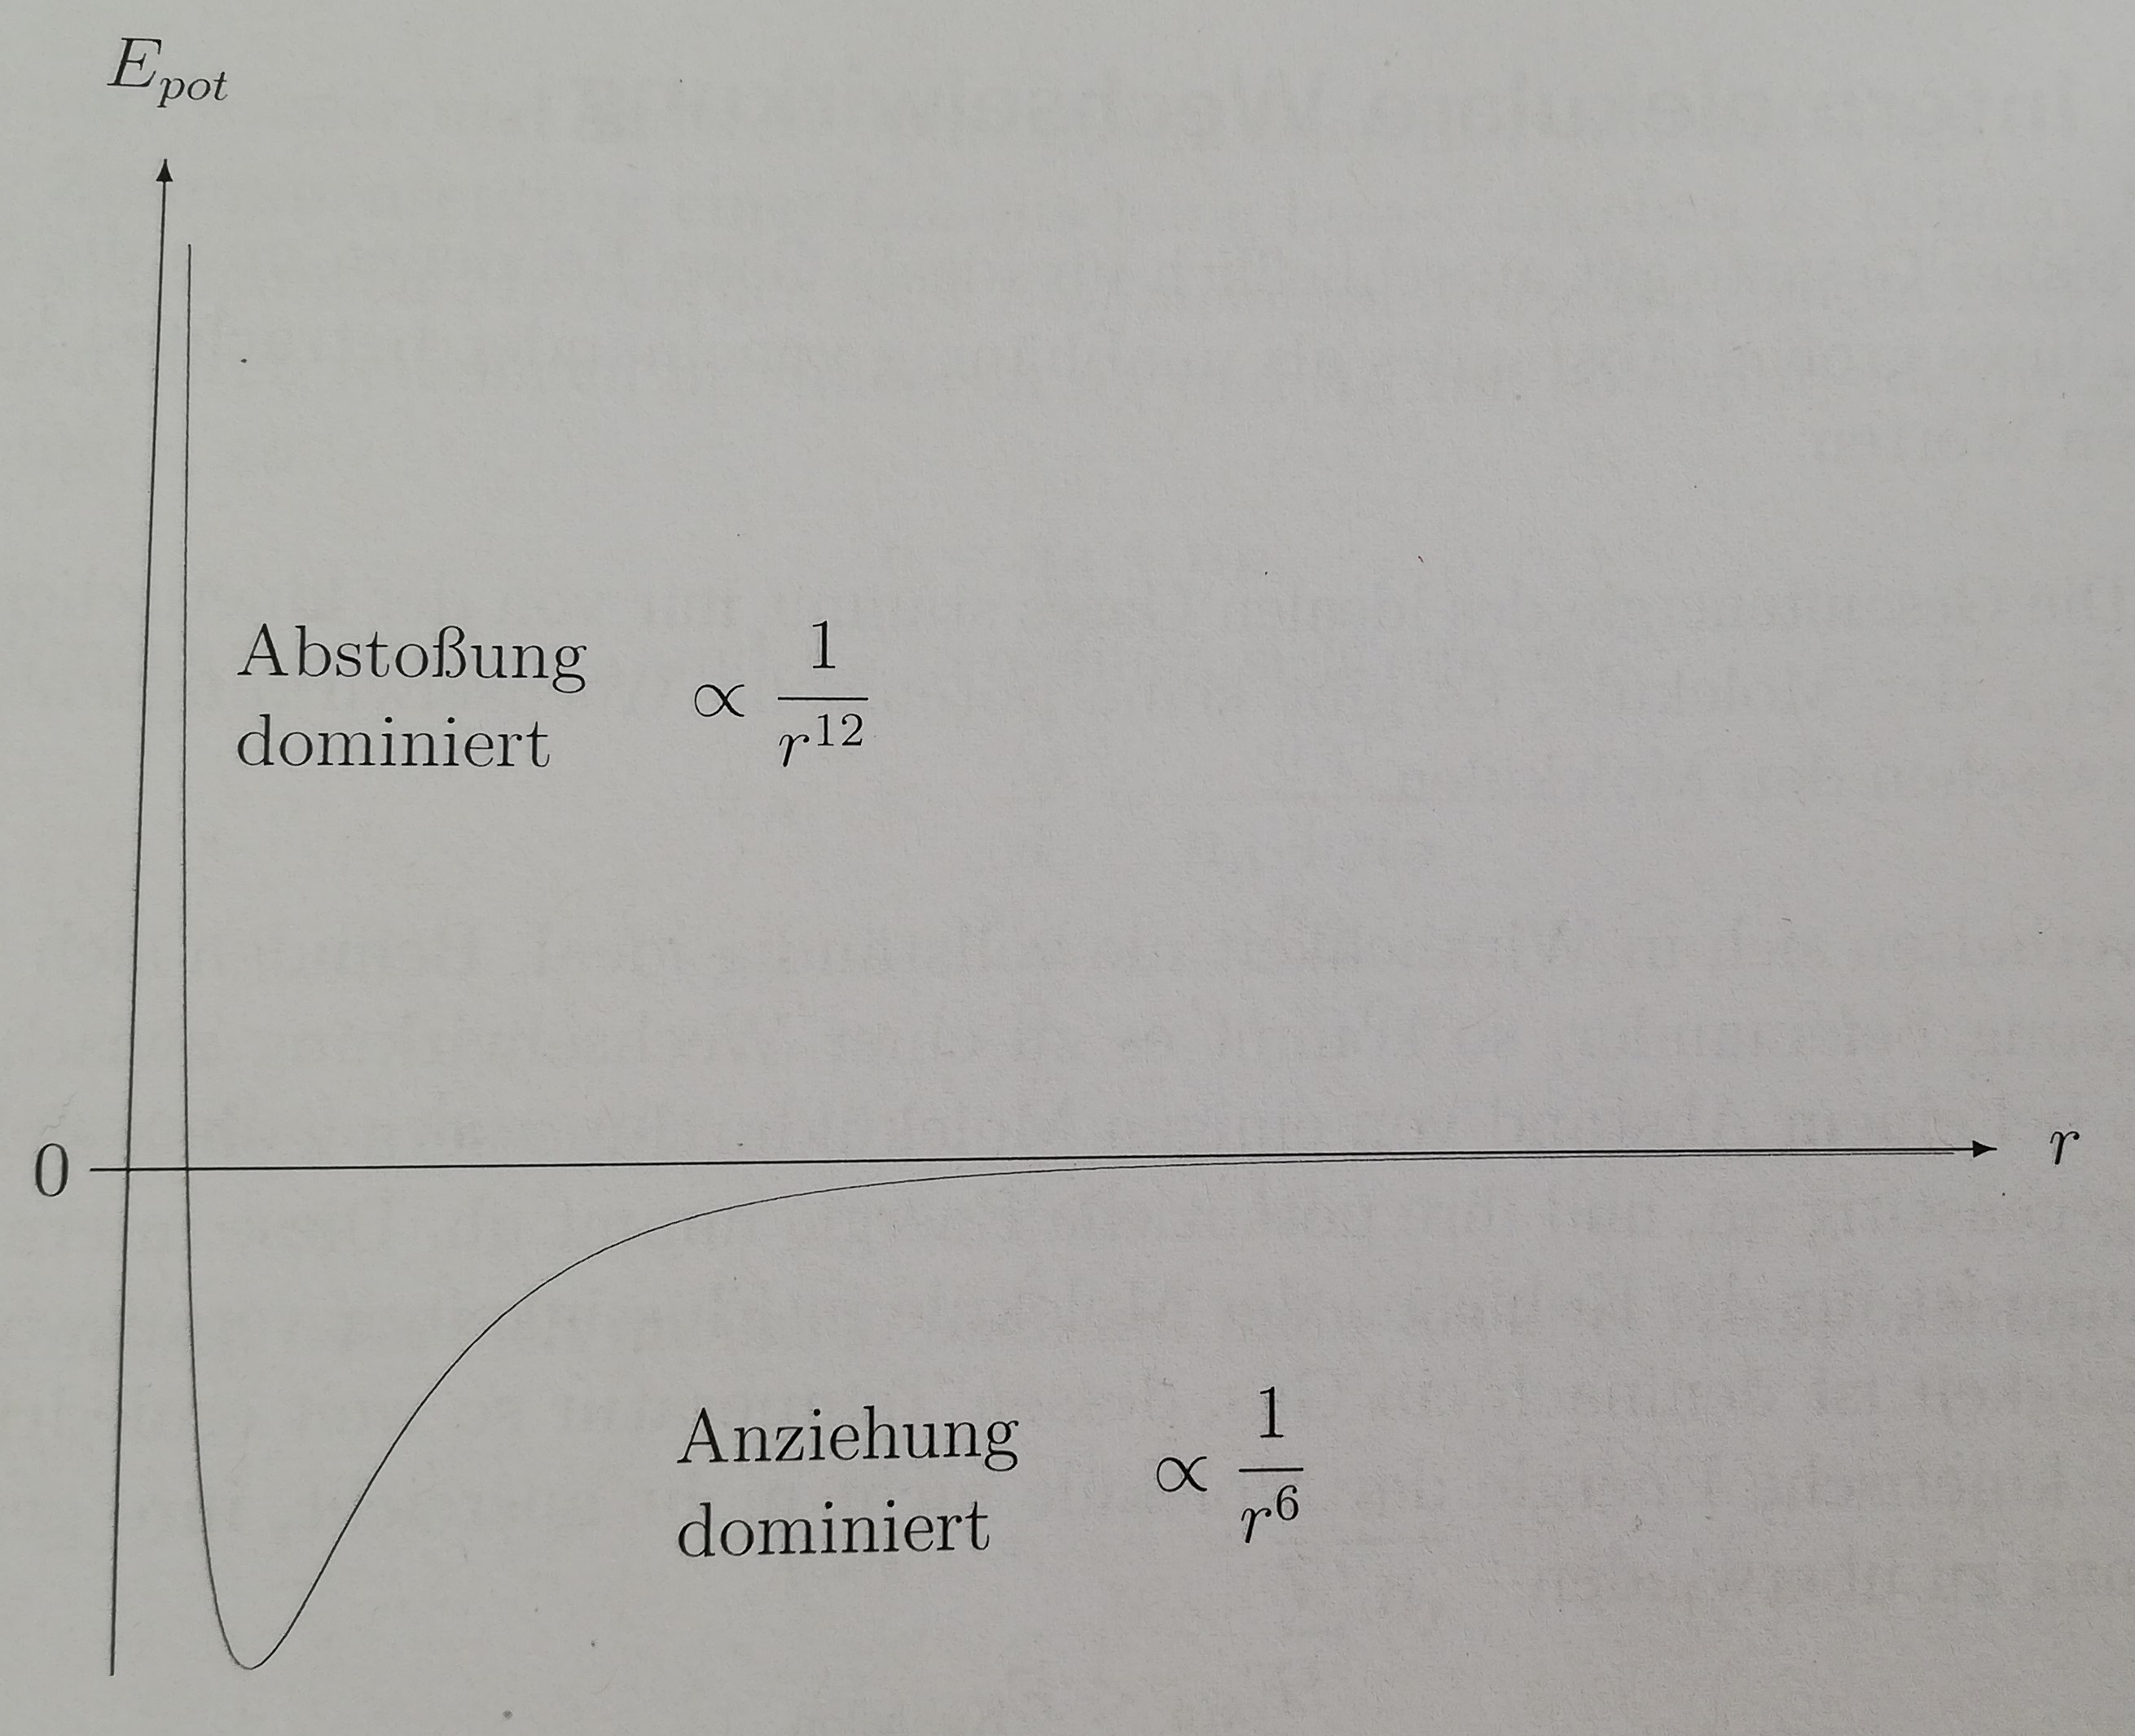
\includegraphics[scale = 0.135]{Bilder/LennardJones.jpg}
    \caption{Skizze des Lennard-Jones-Potentials \protect \footnotemark}
    \label{bild:LJP}
\end{figure}
\footnotetext{\cite{Haefner2019}, S.94}

Diese Wechselwirkungen üben eine Kraft auf den Cantilever aus, der sich infolgedessen verbiegt. Diese Verbiegung wird über einen 
Laserstrahl detektiert, der auf den Cantilever gerichtet ist. Verbiegt sich dieser, so wird auch der Strahl des Lasers unter einem anderen 
Winkel abgelenkt, was ausgewertet werden kann (\cite{Haugstad2012}, S.5). Ein schematischer Aufbau ist in Abb. \ref{bild:Aufbau} zu sehen.

\begin{figure}[h]
    \centering
    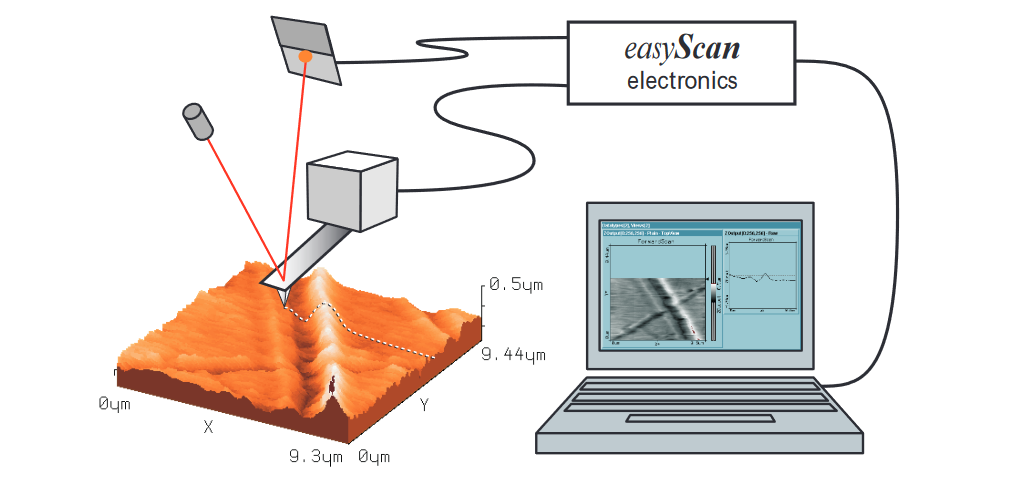
\includegraphics[scale = 0.45]{Bilder/AufbauAFM.png}
    \caption{Schematischer Aufbau eines Rasterkraftmikroskops \protect \footnotemark}
    \label{bild:Aufbau}
\end{figure}
\footnotetext{\cite{easyScan2003}, S.6}

Duch das Funktionsprinzip über die Detektion von Wechselwirkungen sind bei der AFM auch keine besonderen Anforderungen an die Probe 
gestellt. Sie müssen insbesondere nicht leitfähig oder im Vakuum sein. \footnotemark \, Dennoch sollten sie frei vor Verunreinigungen sein 
und vor Feuchte geschützt werden; zudem sollte die Probe zu der verwendeten Spitze passen. 
\footnotetext{Eine AFM im Vakuum liefert dennoch bessere Ergebnisse; für die meisten Zwecke ist eine Untersuchung an der Luft aber 
vollkommen ausreichend}
Die Auflösung wird durch den Krümmungsradius der Spitze und die 
Oberflächenbeschaffenheit der Probe bestimmt und beträgt in der Regel 0.1-10\,nm. Die AFM erreicht also wessentlich höhere Auflösungen als optische Mikroskope. 
Die Spitzenform kann bestimmt werden, indem eine abriebsfeste, scharfkantige Oberfläche bekannten Profils abgerastert wird. In der Praxis werden dazu meist so genannte 
Tipchecks verwendet. \footnotemark \, Alternativ kann die Spitze auch im REM untersucht werden.\\
\footnotetext{\url{https://www.microtonano.com/de/AFM-Tip-Check-und-Test-Probe.php}}


\newpage


\section{Verwendete Modi}
\label{sec:Modi}
Bei der AFM gibt es einige Betriebsmodi; die im Versuch verwendeten sollen hier kurz erläutert werden.

\subsection{Contact Mode}
Im Contact Mode hat die Spitze des Cantilevers dauerhaft Kontakt mit der zu untersuchenden Probe. Man unterscheidet dabei wiederum zwei Modi: \\
Der Constant Hight Mode ist der einfachster aller Modi. In diesem wird der Cantilever auf einer konstanten Höhe über die Probe gefahren. 
Eine Regelung ist nicht nötig. \footnotemark \\
Im Constant Force Mode wird nicht die Höhe über der Probe, sondern die Kraft, die auf die Spitze wirkt, konstant gehalten. Diese wird 
über den sog. Setpoint eingestellt. Zur Beibehaltung der Kraft ist ein PID-Regler notwendig. (\cite{Rieger2013}, S.8)\\
\footnotetext{\url{https://www.nanosurf.com/en/support/afm-modes-overview/contact-modes}, Stand: 23.09.21}
Obwohl der Contact Mode leicht zu realisieren ist, hat er einige Nachteile. So ist durch den dauerhaften Kontakt die Abnutzung der Spitze 
vergleichsweise hoch; zudem kann diese bei plötzlichen Erhebungen oder schlecht gewählten Einstellungen leicht abbrechen. (\cite{Vesely2017}, S.26)

\subsection{Non-Contact Mode}
Im Non-Contact- oder Tapping-Mode (je nachdem ob die Spitze die Probe nie berührt oder kurz antippt) wird der Cantilever mit einer 
konstanten Frequenz nahe seiner Resonanzfrequenz zum Schwingen angeregt. Diese wird wieder über einen PID-Regler gehalten. 
Die Wechselwirkungen zwischen Probe und Spitze bewirken zum einen eine Änderung der Schwingungsamplitude, über die topographische 
Erkenntnisse gewonnen werden können. (\cite{Vesely2017}, S.26). Zum anderen ergibt sich auch eine Phasenverschiebung, die dazu genutzt 
werden kann, Eigenschaften der Probe zu bestimmen (Dichte etc.). \footnotemark \, Der Cantilever kann im Non-Contact Mode als harmonischer Oszillator beschrieben werden. 
Seine Amplitude ergibt sich also nach 
\begin{equation*}
    A(\omega) = \frac{A_0 k}{\sqrt{m^2(\omega_0^2 - \omega^2) + \omega^2 \gamma^2}},
\end{equation*}
mit Federkonstante $k$, Masse $m$, Resonanzfrequenz $\omega_0$ und Dämpfungskoeffizient $\gamma$. Der Setpoint (in Prozent) gibt an, welcher Bruchteil der ungedämpften 
Schwingungsamplitude gehalten wird.
\footnotetext{\url{https://www.nanosurf.com/en/support/afm-modes-overview/dynamic-modes}, Stand: 23.09.21}
 
\section{Regler}

Regler oder Regelkreise sind wichtige Bestandteile von vielen Messapparaturen. Dabei ist ein Regler im Allgemeinen ein Objekt, welches 
ein Eingangssignal $V_e$ aufnimmt, dieses auf eine Art verarbeitet und dann ein Ausgangssignal $V_a$ ausgibt. Das Eingangssignal könnte 
beispielsweise ein Signal eines Sensors sein und das Ausgangsignal könnte der Steuerung eines Bauelements dienen. Dabei gibt es klassisch einige Elemente, die 
oft in Reglern enthalten sind. Diese heißen auch 'Glieder'.

\subsection*{P-Glied}

Ein P-Glied ist etwas Ähnliches wie ein Schalter. Wenn eine bestimmte Bedingung erfüllt ist, dann gibt er einen konstanten Wert aus. Er antwortet also mit einer 
Sprungantwort. Die Antwort ist instantan. Alleine ist er in seiner Anwendung sehr begrenzt; kombiniert man ihn aber mit anderen Gliedern wie dem I- oder D-Glied ist dieser hochwirksam.

\subsection*{I-Glied}

Das 'I' im Namen kommt von 'Integrieren'. Dabei tut dieses Glied genau das, was der Name verspricht. Das I-Glied gibt ein Ausgangssignal aus, welches 
proportional ist zur Integration über das Eingangssignal. Dabei ist klar, dass dieses Glied verzögert antwortet zu dem Eingangssignal, weil 
es dauert, bis das Integral entsprechend groß ist.

\subsection*{D-Glied}

Das D-Glied hat nahezu entgegengesetzte Eigenschaften zum I-Glied. Da es als Ausgangsignal ein Signal ausgibt, welches proportional zu Ableitung des 
Eingangssignal ist, reagiert das Glied instantan. Damit kann es Prozesse wie das Einschwingen von langsam reagierenden Elementen verhindern.

\subsection*{Mehrere Glieder}

Oft verwendet man mehrere Glieder additiv, da diese gegenseitig ihr Vorteile zur Geltung bringen. Man sollte jedoch bedenken, dass zu viele Glieder auch das 
Optimieren des Reglers erschweren, da es sehr viele Parameter gibt, die angepasst werden müssen.


\section{Faltung und das AFM}

Generell kann man eine Faltung mit der Formel 

\begin{equation*}
    (f \circledast g)(t) = \int_{\-\infty}^\infty f(\tau)g(t-\tau) d\tau
\end{equation*}
berechnen. Sie lässt sich aber auch grafisch berechnen, indem man die eine Funktion nimmt, an der y-Achse spiegelt und dann übereinander 'schiebt'. 
Die Überlappung der beiden Funktionen ist dann das Ergebnis der Faltung. \\

Die Faltung spielt in vielen Bereichen der Physik eine Rolle, auch beim AFM. Das was man misst, ist eine Faltung der Spitzenform mit der realen Probenoberfläche\footnote{\url{https://www.weizmann.ac.il/Chemical_Research_Support/surflab/peter/condecon/index.html}, Aufgerufen: 5.10.2021}. 
Dies ist insofern auch schlüssig, da man so keine 'Spalten' in der Probe sehen kann, die schmaler als die Spitze sind. Das gleiche Ergebnis erhält man, wenn man faltet, da die Faltung 
zweier Funktionen runder ist als die rundere der beiden Funktionen.
% Leonhard Schatt

\section{Lock-in Verstärker}

Der Lock-in Verstärker ist ein wichtiges Messgerät. Er wird dazu verwendet schache Signale, die normalerweise weit unter dem Rauschen liegen noch aufzulösen.
Dabei detektiert das Eingangssignal phasenempfindlich. Beim Messen eines Gleichspannungssignals wir das Signal von einem Chopper in den rauscharmen Bereich "hochgemischt". 
Dies geschieht, da bei niedrigen Frequenzen das "rosa Rauschen" dominiert. (\cite{Herink2021}) 

\begin{figure}[h]
    \centering
    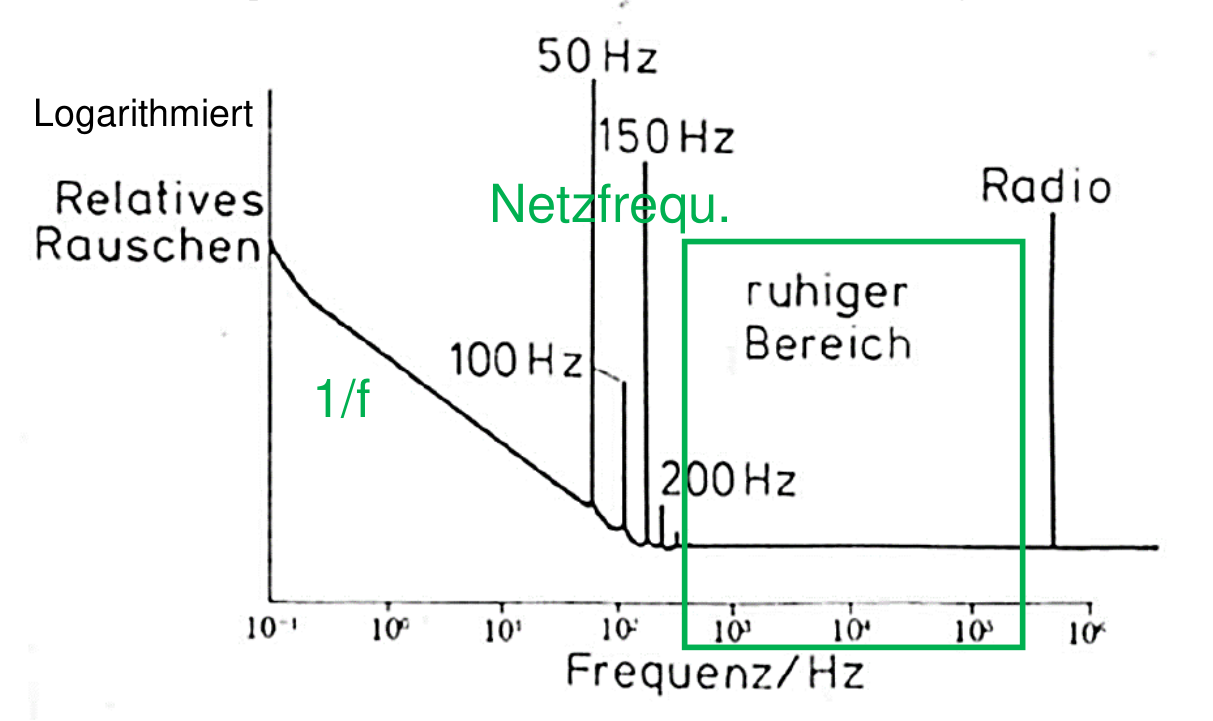
\includegraphics[width = 10cm ]{Bilder/Rauschen.png}
    \caption{Spektrum der Rauschleistung in Abhängigkeit der Frequnez \protect \footnotemark}
\end{figure}
\footnotetext{\cite{Herink2021}}
Im Lock-in Verstärker selbst wird das Signal dann verstärkt und mit einem Referenzsignal $V_R$ gleich der Chopperfrequenz gemischt. Dabei entsteht nach Additiontheoremen für Sinus und Cosinus eine
Differenz- und Summenfrequenz. Dann Filtert man die Differenzfrequenz heraus, indem man einen Tiefpassfilter hinter den Mischer stellt. Im Anschluss wir dann die Spannung abgegriffen. 
Der Vorteil dieses Aufbaus ist, dass die beiden Modulationen durch Chopper und Mischer zusammen wie ein sehr schmalbandiger Filter wirken. Dabei können Bandbreiten von bis zu 0,01Hz erreicht werden. 
Außerdem mittelt sich das Rauschen weg, das es in Beziehung zu $V_R$ unkorreliert ist. Die ausgegebene Spannung hängt jetzt aber noch von der Phasenbeziehung zwischen dem 
modulierten Eingangssignal $V_S$ und dem Referenzsignal $V_R$, das am Mischer ankommt, ab.
\begin{figure}[ht]
    \centering
    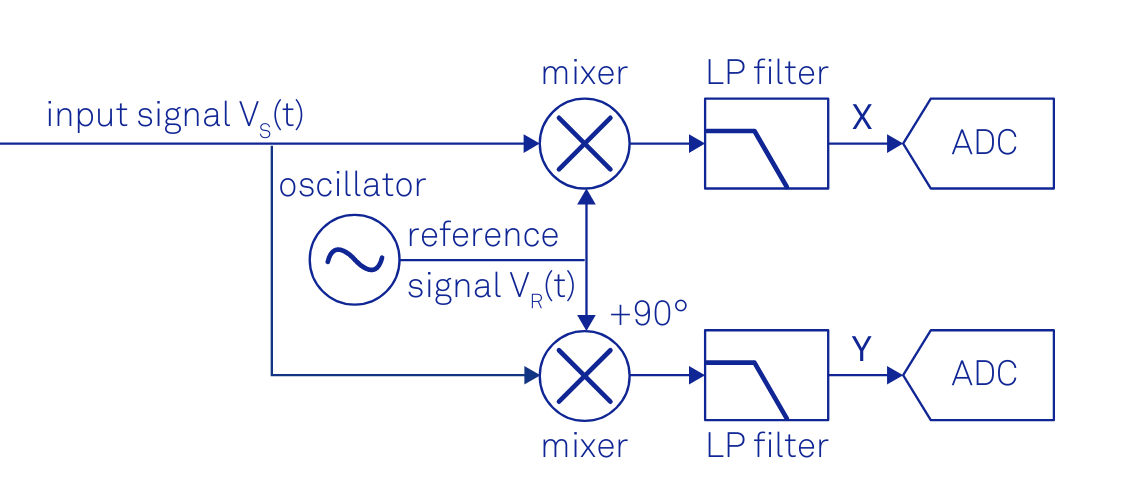
\includegraphics[width = 12cm]{Bilder/Lockin.png}
    \caption{Lock-in Verstärker mit schon moduliertem Eingangssignal $V_S$ \protect \footnotemark}
    \label{lockin}
\end{figure}
\footnotetext{\url{https://www.zhinst.com/sites/default/files/li_primer/zi_whitepaper_principles_of_lock-in_detection.pdf}}
 Deswegen fügt man, wie in Grafik \ref{lockin} zu sehen, einen zweiten Arm ein, on welchen $V_R$ 
um 90° verzögert wird. Aus den beiden Amplituden $X$ und $Y$ berechnet man dann die Amplitude $R$ des Ausgangssignals folgendermaßen:
\begin{equation*}
    R = \sqrt{X^{2}+Y^{2}}
\end{equation*}
  



    % 3.Kapitel Protokoll
    % Charlotte Geiger - Manuel Lippert - Leonard Schatt
% Physikalisches Praktikum

% 3.Kapitel  Protokoll

% Variables
\def\skalierung{0.65}

\chapter{Methodik}
\label{chap:protokoll}
\section{Aufbau}

Der hier verwendete Aufbau besteht aus einem AFM der Marke Nanosurf, einer dazugehörenden Steuerelektronik und einem Computer mit dem 
Programm  'AFM  Nanosurf  Easy  Scan  2'. An diesem kann der Messbereich, der Setpoint, die Zeit pro Zeile und die Anzahl der Zeilen und 
Punkte pro Zeile festgelegt werden. Bilder zum Versuchsaufbau befinden sich im Anhang \ref{section:AnhangAufbau}. \\

\section{Versuchsdurchführung}

Eine Durchführung läuft folgendermaßen ab:\\
Die Probe wird aus ihrer Schachtel genommen und auf die magnetische Platte gegeben. Dann wird mit Hilfe von Millimeterschrauben die Probe unter den Cantilever gefahren. 
Dort wird der Cantilever manuell abgesenkt bis man den Schatten des Cantilevers auf dem Präparat in der Kamera sieht. Danach lässt man den Computer den Cantilever 
automatisch auf die richtige Distanz fahren. Dies geschieht durch eine PI(D)-Regler Schaltung, welche schon voreingestellt war. \\
Anschließend drückt man, nachdem man die entsprechenden Größen eingegeben hat, 'Start' und die Messung läuft von alleine ab. Die Einstellung zur jeweiligen Messung sind unten 
vermerkt.\\
Danach speichert man die Messung als nid-File. Den Angleich der X-Y-Ebene muss man hier nicht manuell durchführen. Diesen übernimmt das Programm automatisch.


\subsection*{Eichgitter}
\begin{center}
    \centering
    \begin{tabular}{l|r}
        Modus & Contact Mode \\
        Image size & 62,65 $\mu$m \\
        Time / Line & 2s \\
        Points/Line & 512\\
        Setpoint & 15 nN \\
        P-Gain & 10000 \\
        I-Gain & 1000 \\
        D-Gain & 0 \\
        
    \end{tabular}
\end{center}

\subsection*{CD-Presswerkzeug}
\subsubsection*{50$\mu$m}
\begin{center}
    \centering
    \begin{tabular}{l|r}
        Modus & Contact Mode\\
        Image size & 50,00 $\mu$m \\
        Time / Line & 2s \\
        Points/Line & 512\\
        Setpoint & 15 nN \\
        P-Gain & 10000 \\
        I-Gain & 1000 \\
        D-Gain & 0 \\
        
    \end{tabular}
\end{center}

\subsubsection*{20$\mu$m}

\begin{center}
    \centering
    \begin{tabular}{l|r}
        Modus & Contact Mode\\
        Image size & 19,34 $\mu$m \\
        Time / Line & 2s \\
        Points/Line & 512\\
        Setpoint & 15 nN \\
        P-Gain & 10000 \\
        I-Gain & 1000 \\
        D-Gain & 0 \\
        
    \end{tabular}
\end{center}

\subsection*{Nanotubes}
\subsubsection*{15$\mu$m}

\begin{center}
    \centering
    \begin{tabular}{l|r}
        Modus & Contact Mode\\
        Image size & 15,00 $\mu$m \\
        Time / Line & 1,3s \\
        Points/Line & 512\\
        Setpoint & 3,02 nN \\
        P-Gain & 10000 \\
        I-Gain & 1000 \\
        D-Gain & 0 \\
        
    \end{tabular}
\end{center}

\subsubsection*{2$\mu$m}

\begin{center}
    \centering
    \begin{tabular}{l|r}
        Modus & Contact Mode\\
        Image size & 2,168 $\mu$m \\
        Time / Line & 1,3s \\
        Points/Line & 512\\
        Setpoint & 3,02 nN \\
        P-Gain & 10000 \\
        I-Gain & 1000 \\
        D-Gain & 0 \\
        
    \end{tabular}
\end{center}

\subsection*{Goldcluster}

\subsubsection*{2,5 $\mu$m}
\begin{center}
    \centering
    \begin{tabular}{l|r}
        Modus & Non-Contact Mode\\
        Image size & 2,5 $\mu$m \\
        Time / Line & 1s \\
        Points/Line & 512\\
        Setpoint & 60\% \\
        P-Gain & 10000 \\
        I-Gain & 1000 \\
        D-Gain & 0 \\
        
    \end{tabular}
\end{center}

\subsubsection*{1,5 $\mu$m}
\begin{center}
    \centering
    \begin{tabular}{l|r}
        Modus & Non-Contact Mode\\
        Image size & 1,5 $\mu$m \\
        Time / Line & 1s \\
        Points/Line & 512\\
        Setpoint & 70\% \\
        P-Gain & 10000 \\
        I-Gain & 1000 \\
        D-Gain & 0 \\
        
    \end{tabular}
\end{center}

\subsubsection*{0,375 $\mu$m}
\begin{center}
    \centering
    \begin{tabular}{l|r}
        Modus & Non-Contact Mode\\
        Image size & 0,375 $\mu$m \\
        Time / Line & 1s \\
        Points/Line & 512\\
        Setpoint & 70\% \\
        P-Gain & 10000 \\
        I-Gain & 1000 \\
        D-Gain & 0 \\
        
    \end{tabular}
\end{center}

\subsection*{Oberflächengitter}

\begin{center}
    \centering
    \begin{tabular}{l|r}
        Modus & Non-Contact Mode\\
        Image size & 20 $\mu$m \\
        Time / Line & 1,75s \\
        Points/Line & 512\\
        Setpoint & 60\% \\
        P-Gain & 10000 \\
        I-Gain & 1000 \\
        D-Gain & 0 \\
        
    \end{tabular}
\end{center}

\subsection*{PSPMMA}

\begin{center}
    \centering
    \begin{tabular}{l|r}
        Modus & Non-Contact Mode, Phase Contrast\\
        Image size & 2 $\mu$m \\
        Time / Line & 1s \\
        Points/Line & 512\\
        Setpoint & 70\% \\
        P-Gain & 10000 \\
        I-Gain & 1000 \\
        D-Gain & 0 \\
        
    \end{tabular}
\end{center}




\section{Geräte und Fehler}

Rasterkraftmikroskop: Inventarnummer: 88459\\
Steuerelektronik: Inventarnummer: 88080\\
Cantilever (Contact Mode): NANOSENSORS type PPP-CONT nachdeR-C, S/N 78932F10L995, vom 31.7.14, Set 5\\
Cantilever (Non-Contact): NANOSENSORS, Type PPP-NCLR-10, S/N 66017F4L734
Eichgitter: Nummer: BT00250, x-y-Periodizität: 10,0 $\mu$m, z-Höhe: 119nm, Batch: 2003-03-29.2
Diverse Proben: Nanosurf Extended Sample Kapitel\\
Oberflächengitter: Gitter(1.9.14)



% Einbindung des Protokolls als pdf (mit Seitenzahl etc.)
% Erste Seite mit Überschrift
%\includepdf[pages = 1, landscape = false, nup = 1x1, scale = \skalierung , pagecommand={\thispagestyle{empty}\chapter{Protokoll}}]
%            {03-Protokoll/Protokoll.pdf}
% Restliche Seiten richtig skaliert
%\includepdf[pages = -, landscape = false, nup = 1x1, scale = \skalierung , pagecommand={}]
%            {03-Protokoll/Protokoll.pdf}

    % 4.Kapitel Versuchsauswertung
    % Matteo Kumar - Leonard Schatt
% Fortgeschrittenes Physikalisches Praktikum
% 4.Kapitel Versuchsauswertung

\chapter{Auswertung und Diskussion}
\label{chap:versuchsauswertung}

% Text

% Input der Teilauswertung je nach Produktion der Nebendateien ohne Ordner
%Matteo Kumar - Leonhard Schatt
% Fortgeschrittenes Physikalisches Praktikum

% Teilauswertung Eichgitter

\section{Vermessung eines Eichgitters}
\subsection{x-y-Verschiebung}
Zuerst soll das Eichgitter vermessen und die Messergebnisse mit den Herstellerangaben verglichen werden. Dazu wird die Aufnahme des AFM mit 
Gwyddion \footnotemark \footnotetext{\url{http://gwyddion.net/}} geöffnet und untersucht.\\
Zur Bestimmung der x-y-Verschiebung werden Strecken über mehrere Raster hinweg und einzelne Raster wie in Abb. \ref{bild:EichWo} gezeigt 
gemessen. 

\begin{figure}[h]
    \centering
    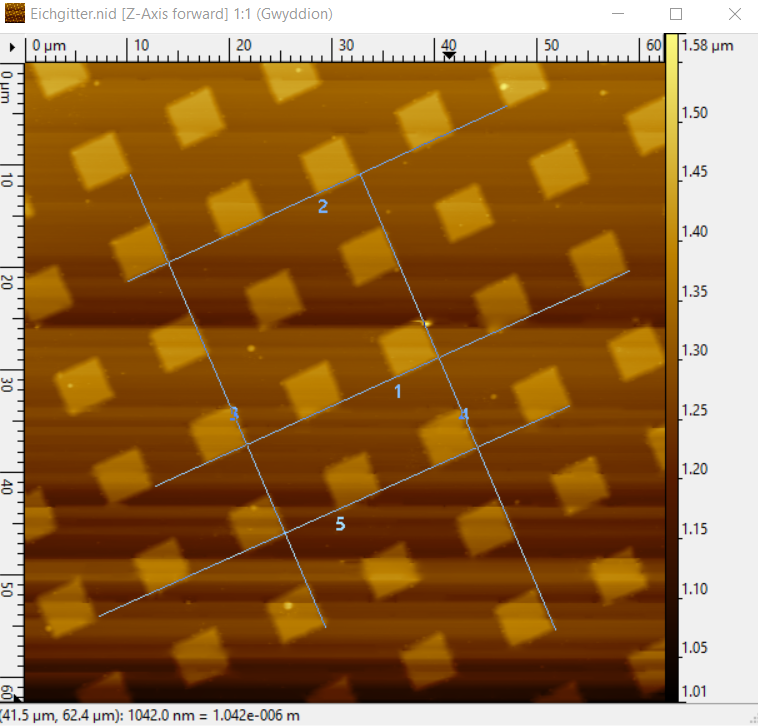
\includegraphics[scale = 0.5]{Bilder/EichGeraden.png}
    \caption{Lage der vermessenen Geraden im Eichgitter}
    \label{bild:EichWo}
\end{figure}
\newpage

Die Längen der Strecken sind:

\begin{center}
    \centering
    \begin{tabular}{l|r r}
        Nummer & Strecke / $\mu m$ & Anzahl Raster \\
        \hline
        1 & 50.9 & 10\\
        2 & 40.8 & 8\\
        3 & 48.2 & 10 \\
        4 & 48.4 & 10 \\
        5 & 50.3 & 10\\
        
    \end{tabular}
\end{center}

Aus den Längen lässt sich der Mittelwert für eine x-y-Versetzung berechnen.

\begin{equation*}
    d_{xy} = 9.942 \mu m
\end{equation*}

Der Hauptfehler dürfte beim Wählen der Start- und Endpunkte 
der zu vermessenden Strecke liegen, da diese nicht sehr gut exakt zu setzen waren. Mithilfe des Vermessungstools wird dieser Fehler auf 
2$\mu m$ pro Strecke abgeschätzt. Nach Fehlerfortpflanzung ergibt sich also:
\begin{equation*}
    s = \sqrt{5}\frac{2 \mu m}{24} = 0.186 \mu m
\end{equation*}

Mit dem internen Fehler des Mikroskops von 1.2\%, ergibt sich für die Versetzung ein Fehler von
\begin{equation*}
    s_d = \sqrt{0.186^2 + (0.012 \cdot 9.942)^2}\, \mu m = 0.22\, \mu m
\end{equation*}

\begin{equation*}
    \textcolor{red}{d_{xy} = (9.94 \pm 0.22) \mu m}
\end{equation*}

Nach Angaben des Herstellers beträgt die Versetzung 10.0 $\mu m$ (s. Protokoll). 
Dieser Wert liegt innerhalb des Fehlers, deshalb kann er als bestätigt angesehen werden. Auffällig ist allerdings, dass sich, 
wenn man die Versetzungen für 'horizontale' (1,2,5) und 'vertikale' (3,4) Strecken getrennt berechnet, unterschiedliche Werte ergeben: 
\begin{equation*}
    d_{xy,h} = 10.14 \mu m, \qquad d_{xy,v} = 9.66 \mu m
\end{equation*}

Dies kann nicht nur Folge von Ungenauigkeiten beim Wählen von den Endpunkten der Strecke sein, dafür ist der berechnete Fehler zu gering. 
Möglich wäre auch noch eine Verkippung des Gitters, sodass die ausgemessenen x-y-Koordinaten nicht exakt der Strecke auf dem Gitter 
entsprechen. In der Tat ist im Profil des Bildes des Eichgitters ein linearer Trend zu erkennen (Abb. \ref{bild:EichKippung}). 
Da die Ergebnisse dennoch gut mit der Theorie übereinstimmen wird an dieser Stelle auf eine Bereinigung verzichtet.

\begin{figure}[h]
    \centering
    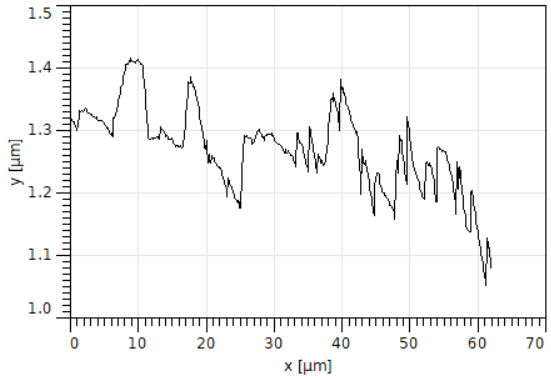
\includegraphics[scale = 0.65]{Bilder/EichKippung.png}
    \caption{Profil des Eichgitters. Ein linearer Trend ist gut zu erkennen - das Gitter ist leicht verkippt.}
    \label{bild:EichKippung}
\end{figure}

\newpage
\subsection{Höhe des Gitters}

Zur Bestimmung der Höhe der Raster wurde ein Höhenprofil von zwei Strecken (s. Abb. \ref{bild:zUebersicht}) erstellt und die Erhöhungen 
vermessen. Die Höhenprofile finden sich in den Abb. \ref{bild:zReihe1} und \ref{bild:zReihe2}. 

\begin{figure}[h]
    \centering
    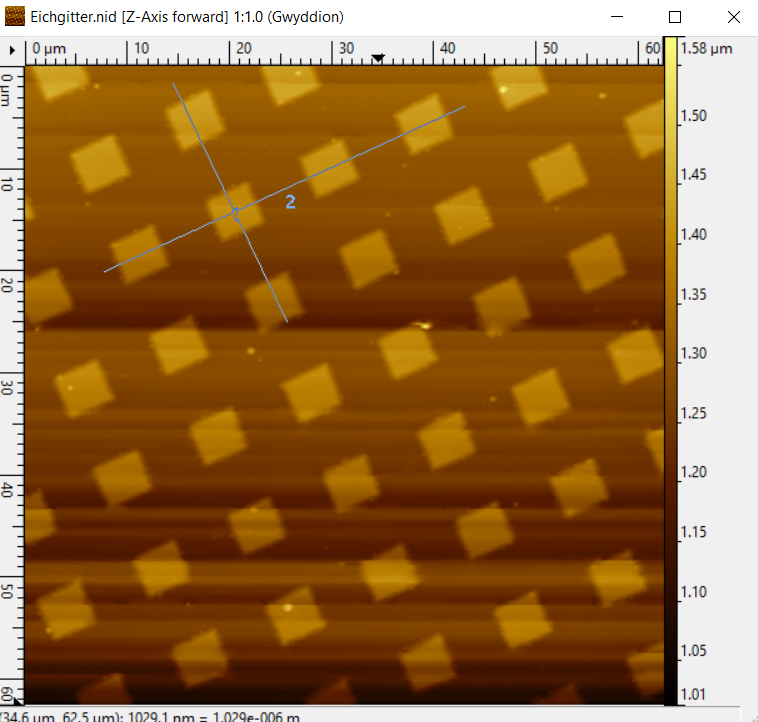
\includegraphics[scale = 0.4]{Bilder/zUebersicht.png}
    \caption{Lage der Geraden zu den Höhenprofilen im Eichgitter}
    \label{bild:zUebersicht}
\end{figure}

\begin{figure}[h]
    \centering
    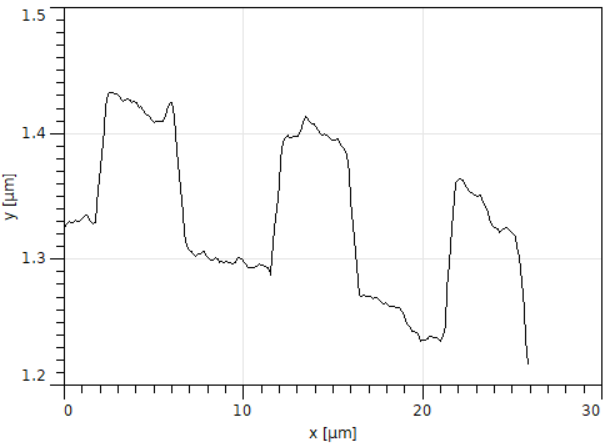
\includegraphics[scale = 0.65]{Bilder/zReihe1.png}
    \caption{Höhenprofil der ersten Geraden}
    \label{bild:zReihe1}
\end{figure}

\begin{figure}[h]
    \centering
    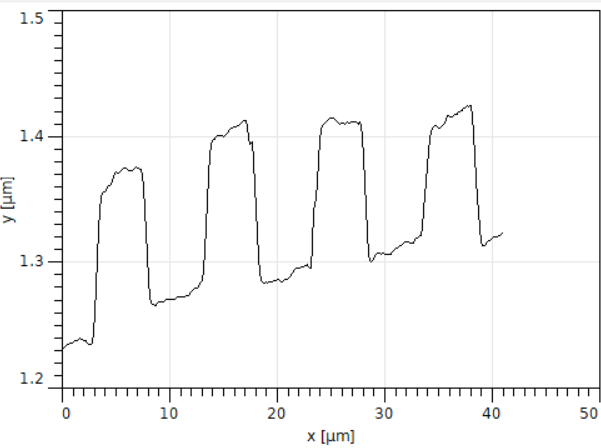
\includegraphics[scale = 0.65]{Bilder/zReihe2.png}
    \caption{Höhenprofil der zweiten Geraden}
    \label{bild:zReihe2}
\end{figure}

\clearpage

Die Höhe der Erhebungen sind: 

\begin{center}
    \centering
    \begin{tabular}{l|r}
        Strecke Reihe 1 /  nm & Strecke Reihe 2 / nm \\
        \hline
        118.0 & 109.6 \\
        107.1 & 119.4 \\
        117.6 & 115.2 \\
        122.3 & 123.7 \\
        119.2 & 128.3 \\
        110.6 & \\
        91.0 & \\
        110.7 & \\
        
    \end{tabular}
\end{center}

Der Mittelwert daraus beträgt $h = 114.823 nm$.
Der Fehler wird hauptsächlich durch die Präzession beim Auswählen der Punkte für die Höhenmessung bestimmt; es war nicht immer klar, 
wo der Anstieg beginnt und endet. Es sei deshalb pro Messung ein Fehler von 5nm angenommen. Über Fehlerfortpflanzung ergibt sich für 
den Fehler des Mittelwerts: 
\begin{equation*}
    s_h = \frac{5}{\sqrt{13}} nm = 1.39 nm
\end{equation*}

Damit ist die Höhe der Erhebungen: 
\begin{equation*}
    \textcolor{red}{h = (114.8 \pm 1.4)nm}
\end{equation*}

Laut Hersteller sollte die Höhe aber 119.0 nm betragen, was außerhalb des Fehlerbereichs liegt (s. Protokoll). Eine Erklärung wäre, dass der Fehler 
zu niedrig abgeschätzt wurde. Wahrscheinlicher ist es aber, dass die Erhöhungen im Laufe der Zeit durch das Vermessen im Contact-Mode 
abgeschliffen wurden. Dafür sprechen auch die an den Helligkeitsunterschieden vor allem in der unteren Hälfte von 
Abb. \ref{bild:zUebersicht} erkennbaren horizontalen Linien über den gesamten Gitterausschnitt. Dies könnten Messfehler des 
AFM sein. Deshalb war auch die Wahl der Strecken für diese Messung nicht ganz einfach, da 
eine Stelle mit möglichst wenig Abnutzung gefunden werden musste. Zum Vergleich ist in Abb. \ref{bild:zUngeeignet} ein dafür 
ungeeignetes Profil zu sehen.

\begin{figure}[h]
    \centering
    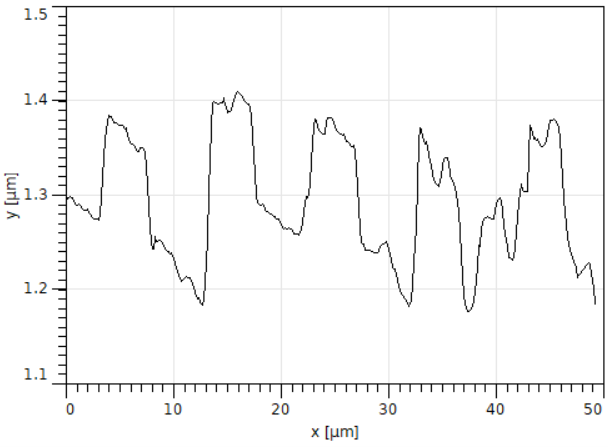
\includegraphics[scale = 0.65]{Bilder/zUngeeignet.png}
    \caption{Ungeeignetes Höhenprofil einer Geraden aus dem Ausschnitt des Eichgitters}
    \label{bild:zUngeeignet}
\end{figure}

\newpage
%Matteo Kumar - Leonhard Schatt
% Fortgeschrittenes Physikalisches Praktikum

% Teilauswertung CD

\section{Untersuchung eines CD-Presswerkzeugs}
\subsection{Bumphöhe}

Zunächst wird der 50$\mu m$-Ausschnitt zur Bestimmung der Bumphöhe untersucht.
Auf Abb. \ref{bild:CD50Linie} ist ein großer heller Fleck am unteren Bildrand zu erkennen. Dies könnte eine Verunreinigung wie z.B. Staub sein. 
Zur Bestimmung der Höhe der Bumps wird das Profil über mehrere Tracks betrachtet. 

\begin{figure}[h]
    \centering
    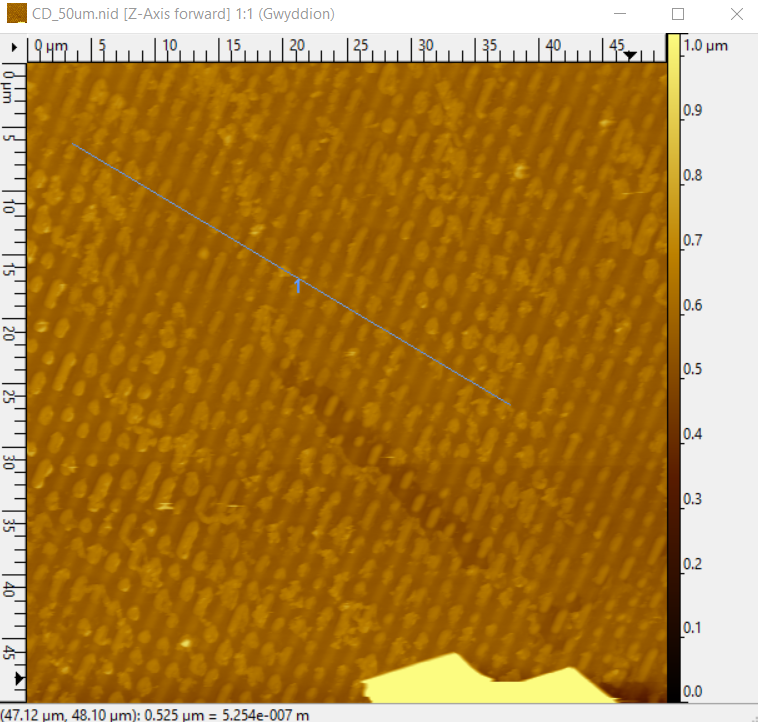
\includegraphics[scale = 0.47]{Bilder/CD50Linie.png}
    \caption{Aufnahme eines CD-Pressswerkzeugs auf 50x50 $\mu$m. Unten ist eine Verunreinigung als heller Fleck zu sehen. Die Strecke 
    für das benutzte Höhenprofil ist ebenfalls eingezeichnet}
    \label{bild:CD50Linie}
\end{figure}

\begin{figure}[h]
    \centering
    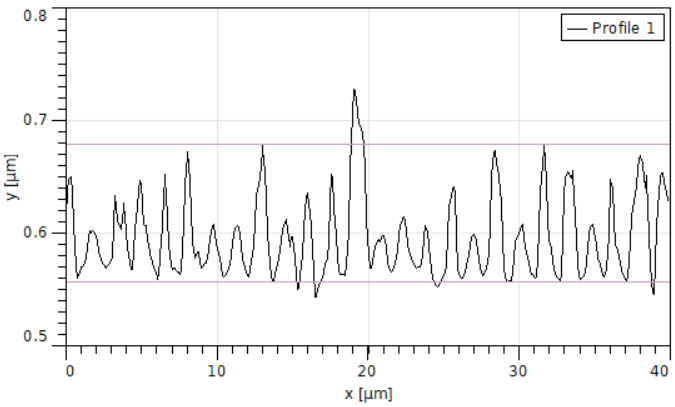
\includegraphics[scale = 0.6]{Bilder/CD50Profil.png}
    \caption{Höhenprofil durch die Bumps des CD-Presswerkzeuges. Als Anhaltspunkt für die Höhe der Bumps dienen die rosafarbenen Linien, die 
    122.2 nm auseinander sind.}
    \label{bild:CD50Profil}
\end{figure}

Die Höhe der Bumps soll mit Hilfe von Abb. \ref{bild:CD50Profil} eingeordnet werden. 
Die rosanen Linien stellen einen Abstand von 122.2 nm dar. Der große Bump hat eine Höhe von 164.4 nm. Der Hersteller 
gibt allerdings Höhen von ca. 200nm an (\cite{SampleKit2007}). Da die Ungenauigkeit des Herstellerwertes nicht bekannt ist, ist eine Einordnung an dieser Stelle 
schwierig. Allerdings ist durchaus zu erkennen, dass die gemessenen Bumps deutlich kleiner sind. Womöglich liegt auch hier bereits eine 
Abnutzung von einigen nm vor.
\newpage

\subsection{Trackabstand}

Nun wird der 20$\mu m$-Ausschnitt betrachtet. Es wird ein Höhenprofil entlang der in Abb. \ref{bild:CD20Linie} eingezeichneten Strecke 
erstellt. Zur Bestimmung des Trackabstandes wird das gesamte Profil über 12 Bumps hinweg gemessen, wie in Abb. \ref{bild:CD20Profil} zu 
sehen. 

\begin{figure}[h]
    \centering
    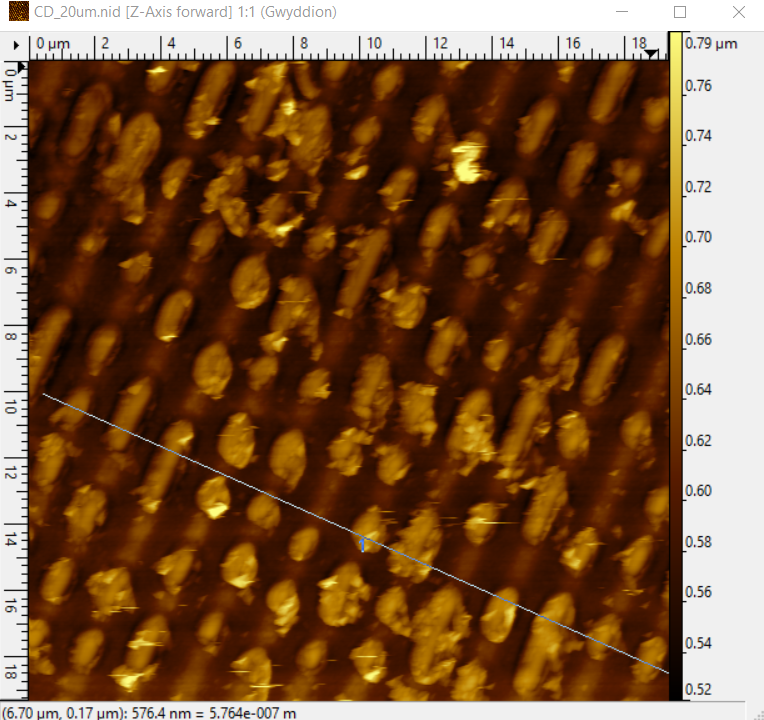
\includegraphics[scale = 0.5]{Bilder/CD20Linie.png}
    \caption{Aufnahme eines CD-Pressswerkzeugs auf 20x20 $\mu$m. Die Strecke 
    für das benutzte Höhenprofil ist ebenfalls eingezeichnet}
    \label{bild:CD20Linie}
\end{figure}

\begin{figure}[h]
    \centering
    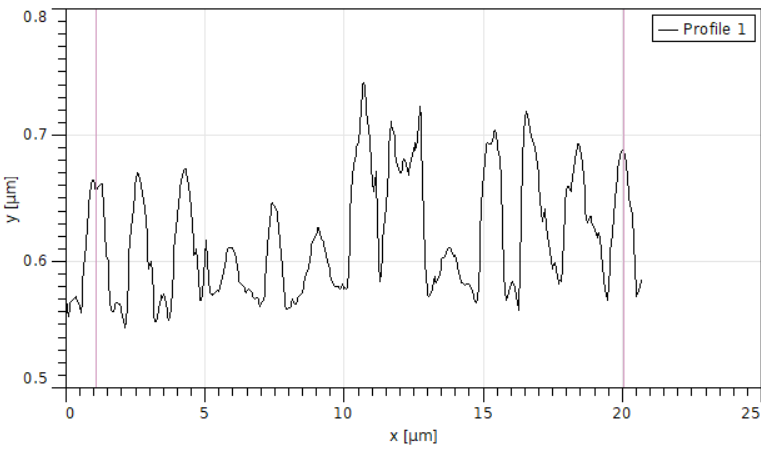
\includegraphics[scale = 0.6]{Bilder/CD20Profil.png}
    \caption{Profil durch die Bumps des Presswerkzeugs. Zur Ermittlung der Trackbreite wurde über 12 Bumps zwischen den rosafarbenen 
    Linien gemessen.}
    \label{bild:CD20Profil}
\end{figure}


Die rosanen Linien stellen einen Abstand von 18.981 $\mu$m dar. Das entspricht einem Trackabstand von $d_{Tr} = 1.582 \mu m$.
Der Fehler ergibt sich aus der Wahl der Veressungslinien, da die Mitte der Bumps nicht exakt bestimmt werden konnte, da die Spitzen und 
der Mittelpunkt zwischen Anstieg und Abfall der Bumps nicht immer übereinstimmen. Deshalb wird der Fehler für beide Linien anhand des 
Profils auf jeweils 0.3 $\mu$m geschätzt. Dies entspricht einem Fehler von 0.05 $\mu$m für den Mittelwert, wodurch sich für den Gesamtfehler ergibt: 
\begin{equation*}
    s = \sqrt{0.05^2 + (1.58 \cdot 0.012)^2}\, \mu m = 0.053\, \mu m
\end{equation*}

Damit ergibt sich der Trackabstand zu

\begin{equation*}
    \textcolor{red}{d_{Tr} = (1.58 \pm 0.06) \mu m}.
\end{equation*}

Der Hersteller gibt einen nominellen Wert von 1.6$\mu$m an (\cite{SampleKit2007}). 
Dieser liegt innerhalb des Fehlers; er wird also durch die Messung bestätigt.

\subsection{Bumplänge}

Als nächstes werden die Längen der Bumps ausgemessen. Dazu wird ein Höhenprofil entlang eines Tracks, wie in Abb. \ref{bild:CD20Laenge} 
gezeigt, angelegt.  

\begin{figure}[h]
    \centering
    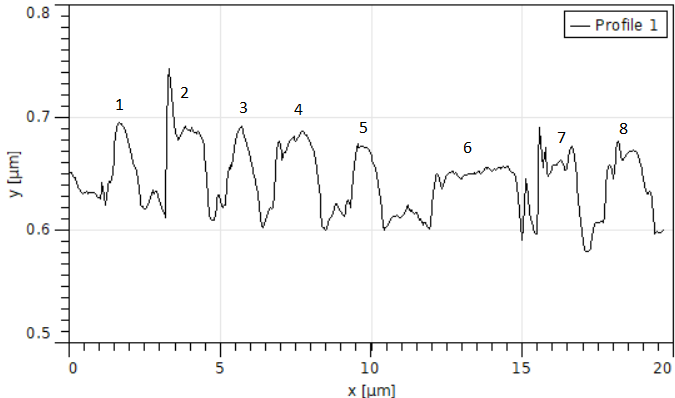
\includegraphics[scale = 0.8]{Bilder/CD20LaengeProfil.png}
    \caption{Profil durch die Bumps des Presswerkzeugs in Längsrichtung.}
    \label{bild:CD20LaengeProfil}
\end{figure}


\begin{figure}[h]
    \centering
    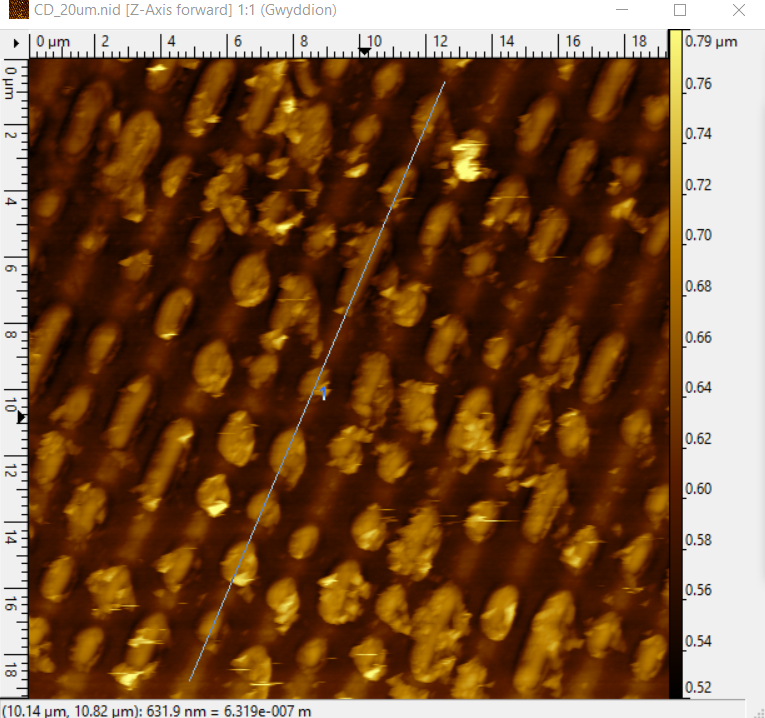
\includegraphics[scale = 0.5]{Bilder/CD20Laenge.png}
    \caption{Strecke entlang eines Tracks, entlang der das Profil zur Bestimmung der Länge der Bumps ermittelt wird.}
    \label{bild:CD20Laenge}
\end{figure}


\newpage

Auf diesem Profil (Abb. \ref{bild:CD20LaengeProfil}) sind acht größere Bumps erkennbar. Von links nach rechts 
sind deren Längen: 

\begin{center}
    \centering
    \begin{tabular}{l|r}
        Nummer Bump (v.l.n.r.) & Länge / $\mu$m \\
        \hline
        1 & 1.28 $\pm$ 1\\
        2 & 1.66 $\pm$ 1\\
        3 & 1.45 $\pm$ 1\\
        4 & 1.95 $\pm$ 1\\
        5 & 1.33 $\pm$ 1\\
        6 & 3.11 $\pm$ 1\\
        7 & 1.74 $\pm$ 1\\
        8 & 1.82 $\pm$ 1\\
        
    \end{tabular}
\end{center}

Die Längen der Bumps in dieser Auswahl liegen also alle im Bereich von 1.2-3.2$\mu$m. Laut Hersteller sollten die Längen in einer Spanne von 
0.8-3$\mu$m liegen (\cite{SampleKit2007}). 
Berücksichtigt man noch die Fehler beim Setzen der Markierungen beim Ausmessen der Bumps (abgeschätzt auf 1$\mu$m 
pro Markierung), so umfasst der angegebene Bereich noch die gemessenen Werte. 
\clearpage
%Matteo Kumar - Leonard Schatt
% Fortgeschrittenes Physikalisches Praktikum

% Teilauswertung Nanoröhrchen

\section{Nanoröhrchen}
Dieser Versuchsteil widmet sich der Untersuchung der Nanoröhrchen. Diese sind Kohlenstoffnanoröhre, welche auf einem Silizium-Waver 
fixiert wurden. Ziel diese Versuchsteiles ist es den Krümmungsradius der Spitze zu bestimmen.
\subsection{Länge und Durchmesser}
\subsubsection*{Länge}
Um die Länge einzelner Nanoröhrchen zu bestimmen, haben wir eine Aufnahme mit 15 $\mu$m als Seitenlängen gemacht. In dieser haben wir uns 
dann angeschaut, welche Längen unterschiedlich lange Kohlenstoffnanoröhren haben. Dazu bestimmt man mit dem Distanzmessen-Tool der Software 
"Gwyddion" die Länge möglichst gerader Nanoröhrchen bestimmt. \\
Die Abbildung \ref{Nanotube20} zeigt die oben genannte Aufnahme. Dabei kann man sehr schön die langgezogenen Fäden sehen. Welche dabei zum Vermessen verwendet wurden, 
kann man Abbildung \ref{Nanotube20Mess} im Anhang entnehmen.

\begin{figure}[h]
    \centering
    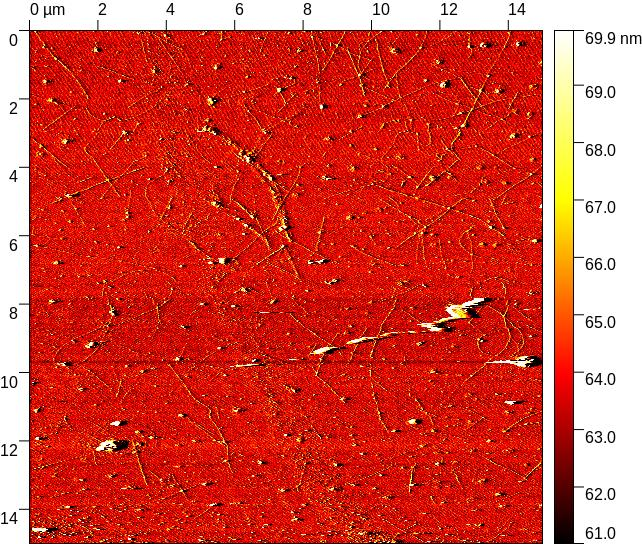
\includegraphics[width = 9cm]{Bilder/Nanotubes/NanoTube15um.jpg}
    \caption{Nanoröhrchen bei einer Bildgröße von 15x15$\mu$m}
    \label{Nanotube20}
\end{figure}

Dabei wurden folgende Werte aus Tabelle \ref{TabLaenge} gemessen. Die Fehlerrechnung kann man bei diesem 
Versuchsteil vernachlässigen, weil die Ablesefehler so groß sind, dass der Fehler des Messgeräts vernachlässigbar klein ist. Der Ablesefehler wird auf 15\% der Länge geschätzt. \\

\begin{table}
    \centering
    \begin{tabular}{lr}
        \toprule
        Röhrennummer &   Länge ($\mu$ m) \\
        \midrule
        0  &  2.883 $\pm$ 0.43 \\
        1  &  2.374 $\pm$ 0.35\\
        2  &  1.334 $\pm$ 0.20 \\
        3  &  3.050 $\pm$ 0.46 \\
        4  &  3.753 $\pm$ 0.56 \\
        5  &   0.860 $\pm$ 0.12\\
        6  &  1.583 $\pm$ 0.24 \\
        7  &  1.896 $\pm$ 0.28 \\
        8  &  1.542 $\pm$ 0.23 \\
        9  &   0.590 $\pm$ 0.075 \\
        10 &   0.464 $\pm$ 0.070 \\
        11 &  4.412 $\pm$ 0.66\\
        \bottomrule
    \end{tabular}
    \caption{Längenmessung der Nanoröhrchen. Der Ablesefehler wird auf 15\% der Länge geschätzt. \\
    }
    \label{TabLaenge}
\end{table}

Man erkennt, dass die Röhren sehr stark in ihrer Länge $l$  variieren.

\begin{equation}
    \textcolor{red}{\frac{l_{Min}}{l_{Max}} = 0.1053209772450975}
\end{equation}

Die maximale relative Unterschied in der Länge $l$ liegt bei einem Faktor 10. Dabei sind die Längen für die langen 
Nanoröhrchen, welche wir gemessen haben, noch nicht mal besonders lang. Diese können in Extremfällen bis zu
einen halben Meter lang werden (\cite{Dagani2002}).

\subsection*{Radius der Röhre}

Man muss sich Nanoröhrchen wie lange Röhren vorstellen, welche eine kreisförmige Grundfläche haben. Von dieser wollen wir nun den 
Radius bestimmen. Da das Abtasten aber einen Kreis mit anderem Radius ergibt muss man statt diesen Radius zu bestimmen, einfach 
den Höhenunterschied der des Hochpunktes der Röhre zum normalen untergrund bestimmen. Leider ist der Untergrund des Silizium-Wavers 
keineswegs glatt; deshalb ist es schwer den Unterschied exakt zu messen. Der Fehler im Ablesen der Werte dominiert den Fehler bei weitem. 
\begin{figure}
    \centering
    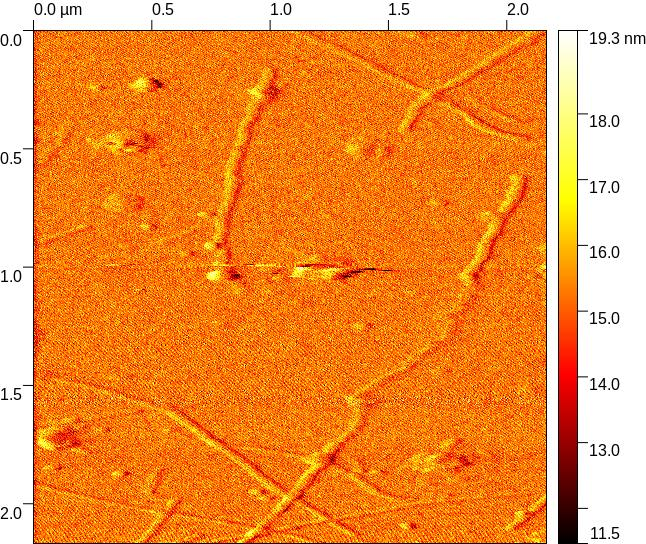
\includegraphics[width = 9cm]{Bilder/Nanotubes/NanoTube2um.jpg}
    \caption{Nanoröhrchen in einer Auflösung mit 512x512 Bildpunkten auf 2x2$\mu$m}
\end{figure}

Zur Bestimmung des Radius wird ein Röhrchen senkrecht mit einer Linie geschnitten. Auf dieser Linie betrachtet man dann das Höhenprofil der Aufnahme. Wir haben dafür die 
Linie, wie in Abbildung \ref{NanoRadius} zu sehen, gewählt. Damit erhält man den Querschnitt, der in Abbildung \ref{NanoQuerschnitt} 
dargestellt wird.

\begin{figure}
    \centering
    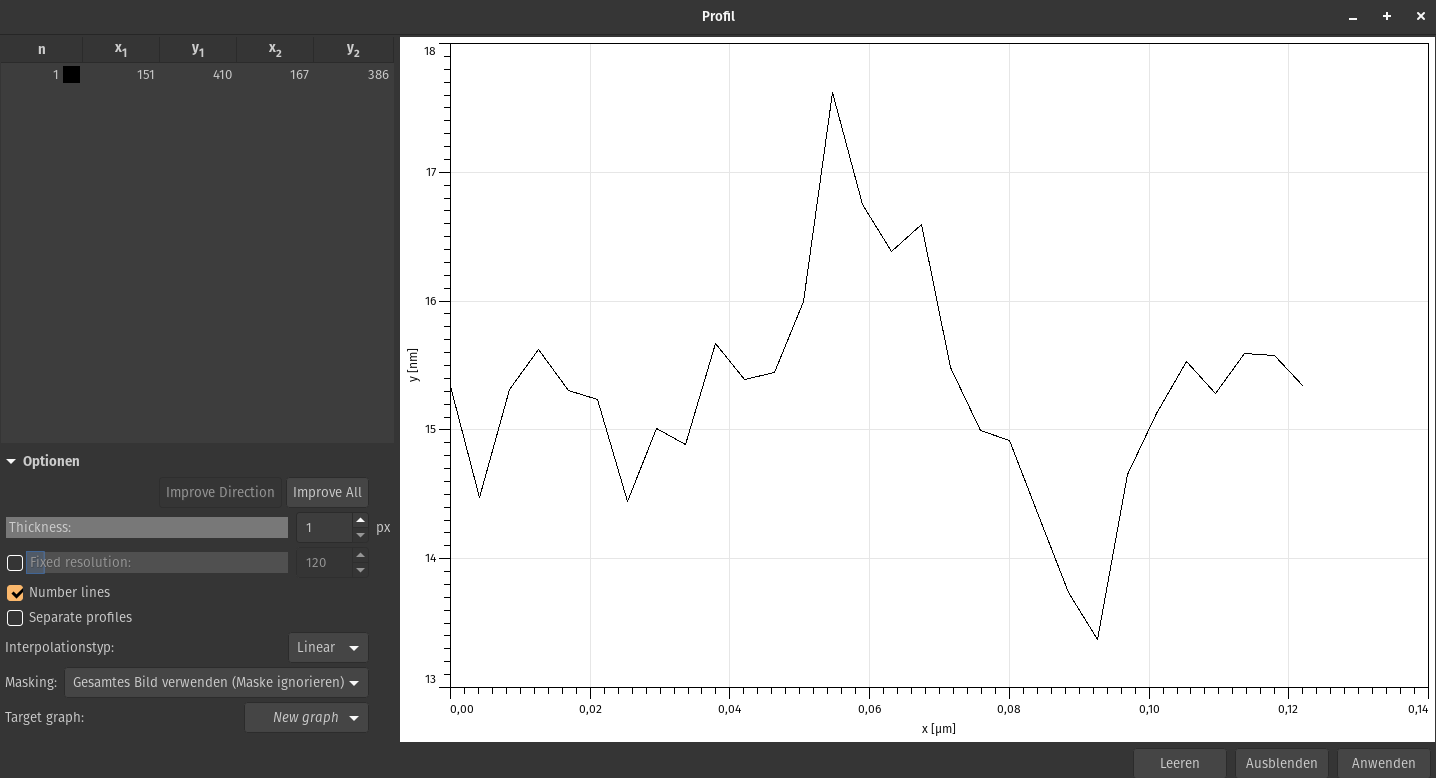
\includegraphics[width = \linewidth]{Bilder/Nanotubes/NanotubesBreiteHoehe.png}
    \caption{Querschnitt eins Kohlenstoffröhrchens}
    \label{NanoQuerschnitt}
\end{figure}

Aus diesem bestimmt man grafisch den Höhenunterschied. Dieser entspricht dann zwei Mal dem Radius $r$ der Röhre. Dabei wird der Fehler 
großzügig mit 15\% des Wertes angegeben.

\begin{equation*}
   r = \frac{\Delta z}{2} = \frac{2,6\mathrm{nm}}{2} = 1,3\mathrm{nm}
\end{equation*}

Durch das halbieren halbiert sich auch der Ablesefehler. 
\begin{equation*}
    \Rightarrow \textcolor{red}{r = (1,300 \pm 0,098)\mathrm{nm}}
\end{equation*}


\subsection{Krümmungsradius der Spitze des Cantilevers}

Wie oben beschrieben sagt die Form der Abtastung etwas über den Krümmungsradius der Spitze des Cantilevers aus. Das wird in Abbildung 
\ref{NanoTip} anschaulich dargestellt.

\begin{figure}
    \centering
    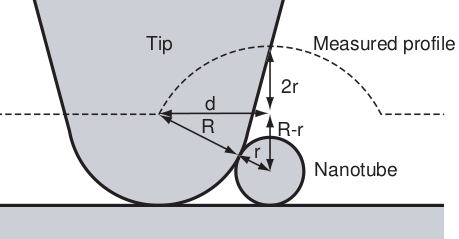
\includegraphics[width = 10cm]{Bilder/Nanotubes/TipGeoNano.png}
    \caption{Zusammenhang Krümmungsradius $R$ der Spitze und Präparatradius $r$ aus der abgebildeten Kontur (\cite[S.46]{SampleKit2007})}
    \label{NanoTip}
\end{figure}

Darau ergibt sich für den Radius der Spitze (\cite[S.47]{SampleKit2007}):\\
\begin{equation}
    R = \frac{d^2}{4r}
\end{equation}
mit $d$, $R$ und $r$ wie in Abbildung\ref{NanoTip} eingezeichnet.

Auch für $d$ setzt man beim Ablesen am besten ein großzügiges Intervall der Unsicherheit von 50\% an, da es schwer ist aus 
dem Rauschen herauszulesen, wo der Peak anfängt. Abgelesen wurde:\\

\begin{equation*}
    2d = 25,0\pm12,5\mathrm{nm} \Rightarrow d = (12,5\pm 6,3) \mathrm{nm} 
\end{equation*}

Daraus ergibt sich mit dem Fehlerfortpflanzungsgesetz:\\

\begin{equation}
    \textcolor{red}{R = (30\pm15) \mathrm{\,nm}}
\end{equation}

Das scheint ein in der Größenordnung realistischer Wert. Die Spitze könnte noch gut sein. Für eine Spitze sind Krümmungsradien zwischen 
10 und 20 nm normal. Die Spitze tendiert aber dazu, etwas abgenutzt zu sein.
\section{Gold}

Bei diesem Versuchsteil soll die Rauheit von Materialien genauer betrachtet werden. Diese gibt an, wie stark die Oberfläche von einer idealen, glatten Oberfläche abweicht. 
Dabei hätte eine ideal glatte Fläche eine Rauheit von 0nm. Je größer diese ist, desto rauer ist die Oberfläche.\\

Hier wird die Rauheit von Gold bestimmt. Dabei wird von einer Goldprobe die Rauheit in drei unterschiedlichen 
Aufnahmegrößen bestimmt. Diese werden dann verglichen und diskutiert.

Die entstehenden Bilder von Gold kann man im Anhang betrachten unter \ref{Gold1}, \ref{Gold2} und \ref{Gold3}.

Dabei erhält man für die Rauheit die folgenden Werte:\\
\begin{center}
    \centering
    \begin{tabular}{lr}
        \toprule
        Seitenlänge des Aufnahmebereichs ($\mu$m) & Rauheit (nm)\\
        \midrule
        2,5 & 1,335\\
        1,5 & 1,468 \\
        0,375 & 1,537\\
    \end{tabular}
\end{center}

Das Ergebnis ist zunächst kontraintuitiv. Man hätte erwartet, dass die Rauheit der Probe sinkt, 
wenn man näher heranzoomt. Aber gerade der gegenteilige Effekt ist zu beobachten. Dies ist damit zu erklären, 
dass bei größeren Ausschnitten das Abtasten nicht präzise genug ist, weil 
die Spitze zu schnell über die Probe lauft. Damit bekommt man kein vollständiges Bild der Probe, sondern nur einen groben Überblick. 
Um diese Hypothese zu überprüfen könnte man noch eine Referenzmessung machen. Bei dieser nimmt man dann den großen Ausschnitt und 
erhöht die Abtastzeit für eine Zeile massiv. Dann sollte man eine höhere Rauheit als die 
drei gemessenen Werte messen.
\clearpage
\section{PS/PMMA}

In diesem Teil der Auswertung wird demonstriert, warum die Information über die Phase beim AFM sehr aufschlussreich sein kann. Hier haben wir 
als Probe ein Gemisch aus Polystyrol und Polymethylmethacrylat. Diese wurden vermischt und dann auf einem Silizium-Waver aufgebracht. 
Jetzt fragt man sich im nachhinein, welches Material welches ist. Aus den topographischen Daten ist das leider nicht mehr ersichtlich. Abgesehen davon kann man auch 
nicht so gut unterscheiden, welcher Teil des Gemisches wo endet (siehe Abbildung \ref{PMMA1}).\\
\begin{figure}[h]
    \centering
    \includegraphics[width = 9cm]{Bilder/PMMA/PSPMMA.jpg}
    \caption{PS/PMMA in der Topographieansicht}
    \label{PMMA1}
\end{figure}

Betrachtet man nun aber das Phasenbild fällt auf, dass die Unterschied eindeutig zu sehen sind. Dabei gibt es sehr dunkle und helle Punkte 
in der Abbildung \ref{PMMA2}.\\

\begin{figure}
    \centering
    \includegraphics[width = 9cm]{Bilder/PMMA/PSPMMAPhase.jpg}
    \caption{Phaseninformation zur selben Aufnahmen wie in Abbildung \ref{PMMA1}}
    \label{PMMA2}
\end{figure}

Das liegt daran, dass beim Phasenkontrastmodus Informationen über die lokale Härte der Probe gesammelt werden. Man kann also 
Rückschlüsse auf die chemische Zusammensetzung beispielsweise machen, welche rein aus dem topographischen Daten nicht ersichtlich waren.\\
Dabei wird der Phasenkontrastmodus vor allem verwendet um einen guten Kontrast im Bild zu erzeugen und qualitative Aussagen zu machen. 
Für quantitative Aussagen ist er oft zu ungenau, da er von zu vielen oft nur ungefähr bekannten Größen wie Federkonstante, unterschiedlichen Kräften und Spitzengeometrie 
abhängt (\cite[S.68]{SampleKit2007}).
Hier kann man beispielweise sagen, dass die hellen Flecken Polystyrol sind, da dieses härter ist als Polymethylmethacrylat\footnotemark.
\footnotetext{\url{https://de.wikipedia.org/wiki/Polymethylmethacrylat}, Eingesehen am 22.09.2021}
%Matteo Kumar - Leonhard Schatt
% Fortgeschrittenes Physikalisches Praktikum

% Teilauswertung Oberflächengitter
\clearpage
\section{Gitterkonstante eines Oberflächengitters}

Als letzes wird noch ein Oberflächengitter vermessen, um dessen Gitterkonstante zu bestimmen. Dazu wird wieder ein Profil entlang der in 
Abb. \ref{bild:OFGitter} eingezeichneten Linie erstellt.

\begin{figure}[h]
    \centering
    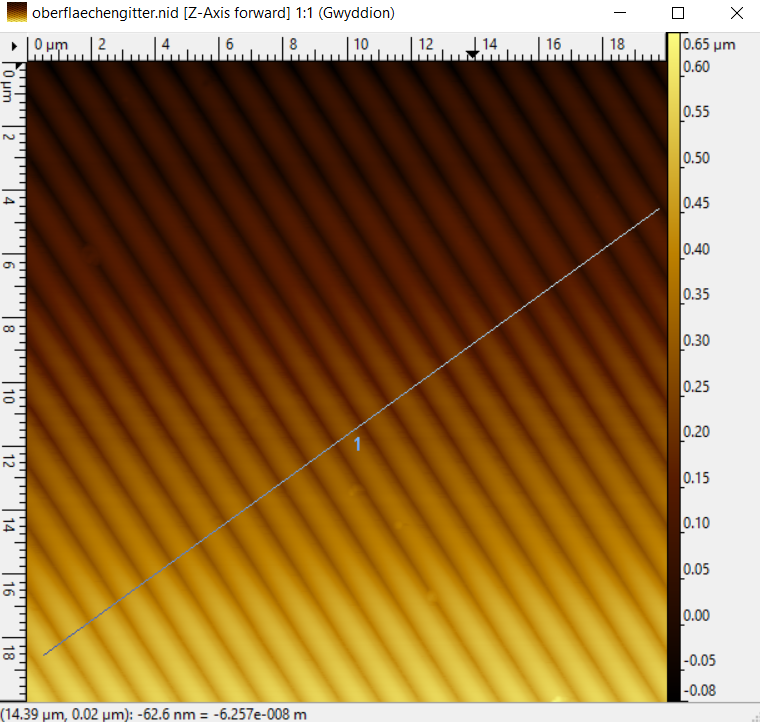
\includegraphics[scale = 0.45]{Bilder/OFGitter.png}
    \caption{Höhenprofil der ersten Geraden}
    \label{bild:OFGitter}
\end{figure}

\begin{figure}[ht]
    \centering
    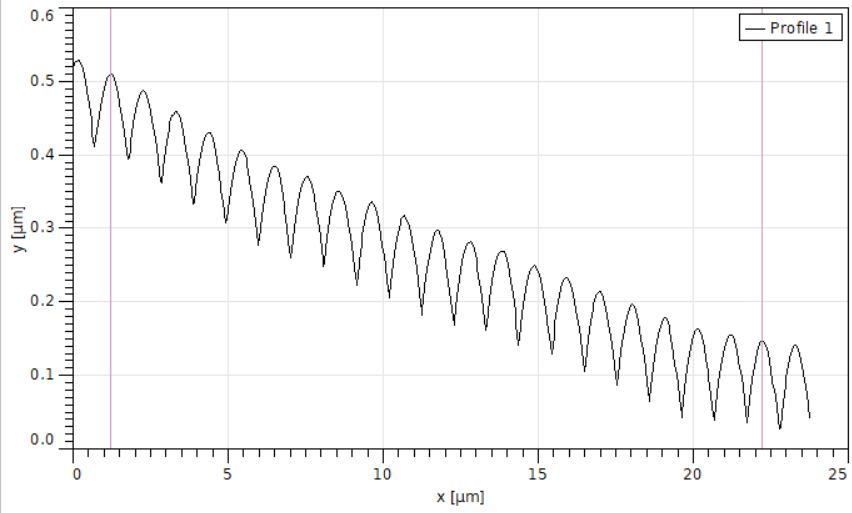
\includegraphics[scale = 0.55]{Bilder/OFGitterProfil.png}
    \caption{Höhenprofil der ersten Geraden}
    \label{bild:OFGitterProfil}
\end{figure}


Anschließend wird das Profil über 20 Kanten hinweg vermessen, wie in Abb. \ref{bild:OFGitterProfil} gezeigt. Die Gesamtlänge beträgt 
21.016 $\mu$m; der Mittelwert beträgt also 1.0508$\mu$m. 
Der Fehler liegt wieder in dem Setzen der Linien, zwischen denen gemessen wurde. Anhand des Abmess-Tools wird dieser auf 0.1$\mu$m pro 
Linie geschätzt. Für den Mittelwert ergibt sich demnach ein Fehler von 0.01$\mu$m. Der Gesamtfehler ergibt sich mit dem internen Fehler also zu
\begin{equation*}
    s = \sqrt{0.01^2 + (0.012 \cdot 1.0508)^2}\, \mu m = 0.016 \mu m
\end{equation*}
Die Gitterkonstante des Oberflächengitters beträgt also:
\begin{equation*}
    \textcolor{red}{g = (1.051 \pm 0.016) \mu m}
\end{equation*}



% etc.

    % 5.Kapitel Fazit
    %Matteo Kumar - Leonard Schatt
% Fortgeschrittenes Physikalisches Praktikum

% 5. Kapitel Einleitung

\chapter{Fazit}
\label{chap:fazit}
Wie in der Einleitung schon beschrieben ist FRET ein wichtiger Effekt, der vor allem in organischen Systemen auftritt. Dieser 
wurde uns in diesem Versuch näher gebracht. Das Auswerten ganzer Bilddateien mit 'Fiji' war auch eine neue Erfahrung, 
welche sicher in späteren Arbeiten noch eine Anwendung finden wird. Des Weiteren haben wir einen guten Einblick zu Fluorophoren bekommen; uns ist nun klar, dass
die Darstellung von leuchtenden Mäusen in biochemischen Laboren eine lächerliche Erfindung der Filmindustrie ist, da die Lebensdauer der angeregten 
Zustände sich im Nanosekundenbereich befindet. 



    % Matteo Kumar - Leonard Schatt
% Physikalisches Praktikum

% Anhang

\appendix

% Text

% Matteo Kumar - Leonard Schatt
% Physikalisches Praktikum

% Anhang A

\chapter{Anhang}
\label{chap:anhangA}
\section{FLIM}

\begin{figure}[h]
    \centering
    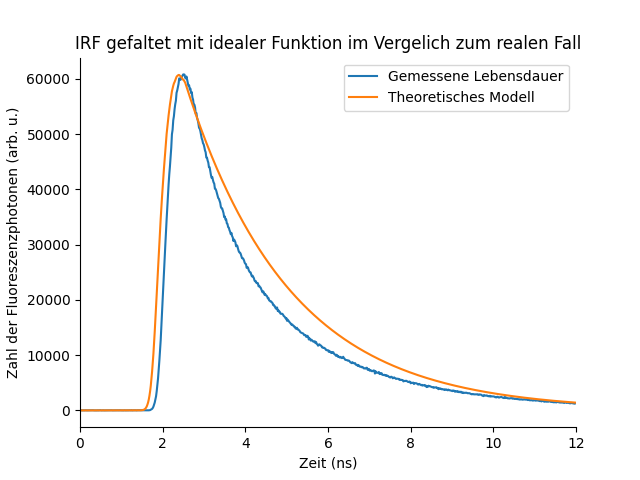
\includegraphics[width = \linewidth]{Bilder/Auswertung/IRFProgConvol.png}
    \caption{Lebensdauer bei Einzelphotonenereignissen und die Faltung der IRF (Programmgeneriert) und dem idealen Signal ($\tau_{YFP}$ unkorrigiert) nach der Totzeit. }
    \label{bild:IRFconvProg}
\end{figure}


\begin{figure}[h]
    \centering
    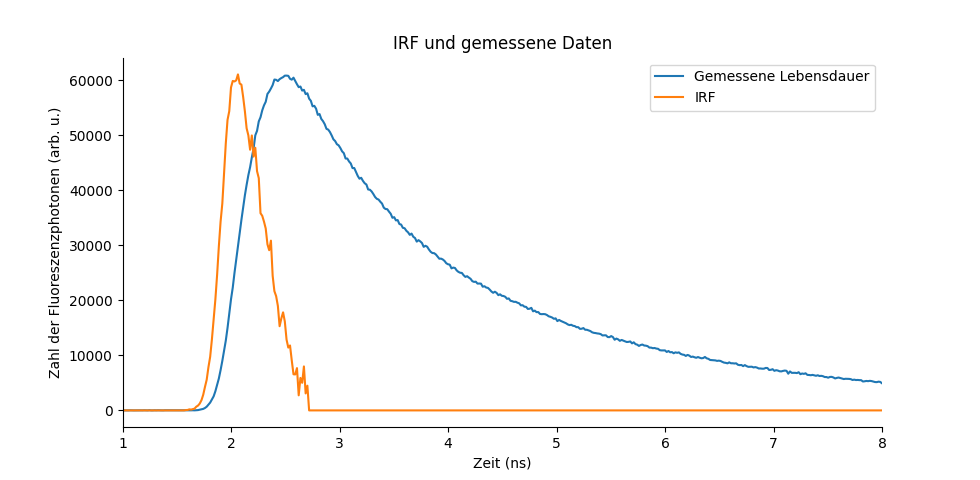
\includegraphics[width = \linewidth]{Bilder/Auswertung/IRFProg.png}
    \caption{ Lebensdauer bei Einzelphotonenereignissen und IRF durch das Programm 'SymPhoTime' generiert. Man sieht eine unsymmetrische Form.}
    \label{bild:IRFProg}
\end{figure}



\clearpage
\section{Protokoll}
\label{section:Protokoll}
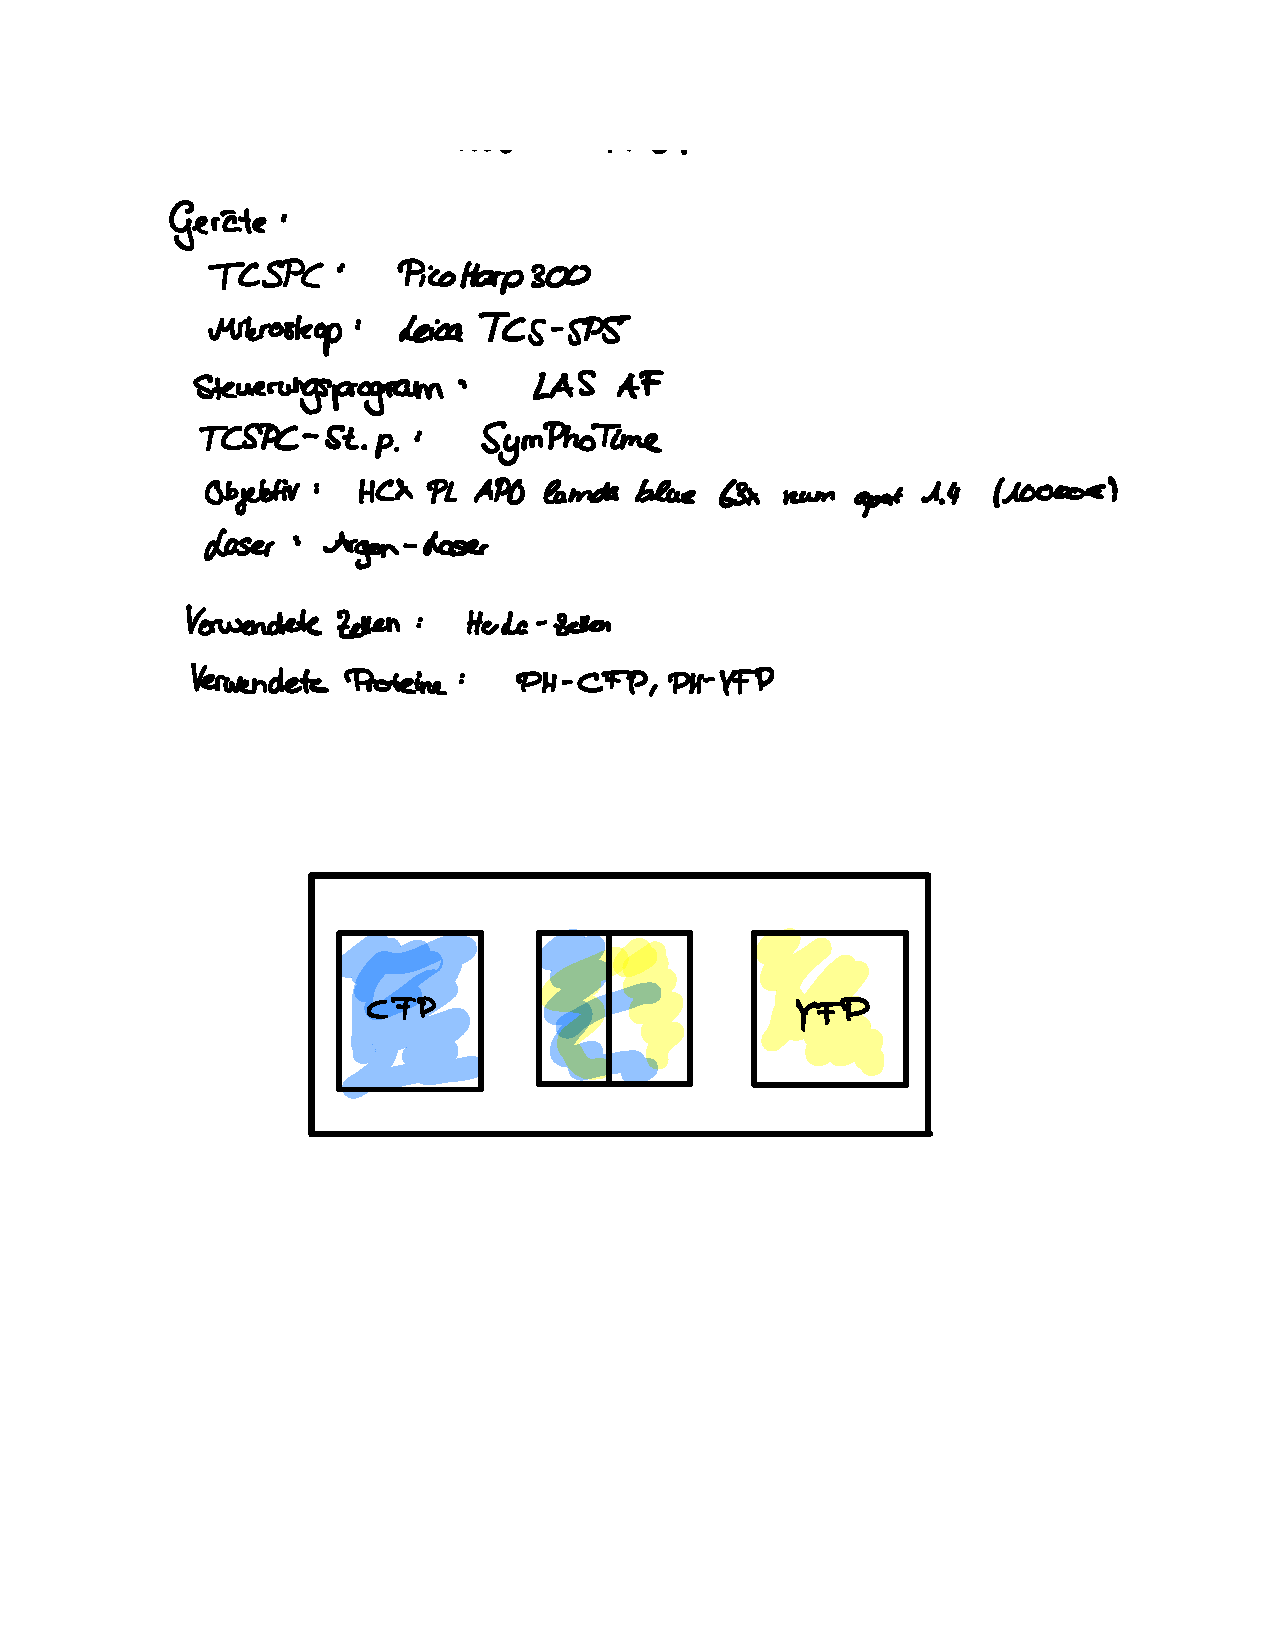
\includepdf[pages = 1-6]{FRETProt.pdf}



    % Literatur
    \bibliographystyle{Auswertung.bst}
    %\nocite{*}
    \bibliography{Auswertung.bib}

\end{document}